\chapter{Appendix \autoref{chap:understanding}}

\section{Implementation details and hyperparameters} \label{app:impl}

We employ two commonly used implementations, one for fast iterations on priming experiments (\href{https://github.com/denisyarats/pytorch\_sac}{https://github.com/denisyarats/pytorch\_sac}) and one for scaling up our experiments to high update ratios (\href{https://github.com/proceduralia/high\_replay\_ratio\_continuous\_control}{https://github.com/proceduralia/high\_replay\_ratio\_continuous\_control}). All experiments in the main sections use default hyperparameters of the high update ratio codebase  unless otherwise specified with minor exceptions.

\begin{table}[H]
    \parbox[t]{.45\linewidth}{
    \label{tab:sharedhparam}
    \centering
    \caption{Shared hyperparameters between priming and high-UTD implementations}
    \begin{tabular}{ | m{3.5cm} | m{2cm}| }
      \hline
      Optimizer & Adam \\ 
      \hline
      Adam $\beta_1$ & $0.9$ \\ 
      \hline
      Adam $\beta_2$ & $0.999$ \\ 
      \hline
      Adam $\varepsilon$ & $1e-8$ \\ 
      \hline
      Actor Learning Rate & $4e-3$ \\ 
      \hline
      Critic Learning Rate & $4e-3$ \\ 
      \hline
      Temp. Learning Rate & $3e-4$ \\ 
      \hline
      Batch Size
      & $256$ \\ 
      \hline
      $\gamma$ & $0.99$ \\
      \hline
      $\tau$ & $0.005$ \\
      \hline
      \# critics & $2$ \\
      \hline
      \# critic layers & $2$ \\
      \hline
      \# actor layers & $2$ \\
     \hline
      critic hidden dim & $256$ \\
     \hline
      actor hidden dim & $256$ \\
     \hline
    \end{tabular}
    \label{tab:shared}
    }
    \hfill
    \parbox[t]{.55\linewidth}{
    \centering
    \caption{Differing hyperparameters between priming and high-UTD implementations}
    \begin{tabular}{ |m{2cm} | m{2.5cm} |  m{2.5cm}| }
     \hline
     & Priming & High UTD \\
     \hline\hline
     Initial \newline temperature & $0.1$ & $1.0$ \\
     \hline
     Target \newline entropy & -action\_dim & -action\_dim / 2 \\
     \hline
     actor log \newline std bounds & [-5, 2] & [-10, 2] \\
     \hline
    \end{tabular}
    }
\end{table}

\section{Additional priming experiments} \label{app:priming}

\subsection{Activation functions}

\begin{figure}[H]
% \captionsetup[subfigure]{font=footnotesize, aboveskip=2pt}
\centering
    \begin{subfigure}[b]{0.8\textwidth}
        \centering
        
\includegraphics[height=0.4cm]{figures/dissecting/priming/elu_priming_base_return_legend.pdf}
    \end{subfigure}\\%
    \begin{subfigure}[b]{0.33\textwidth}
        \centering
        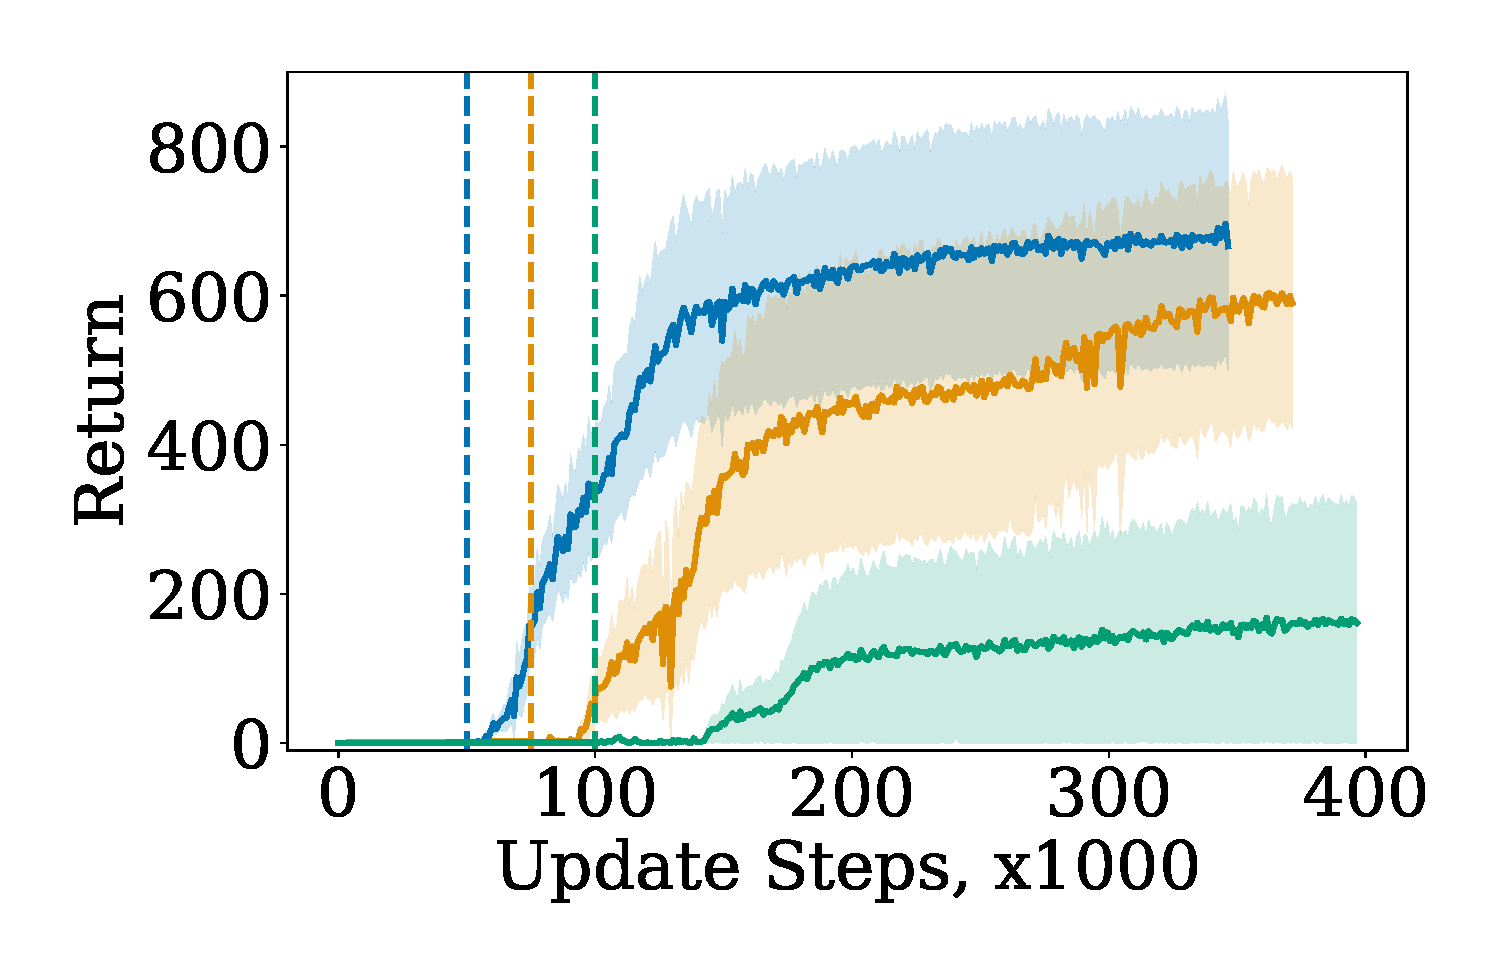
\includegraphics[width=4.7cm, trim=1cm 1cm 1cm 1cm ,clip]{figures/dissecting/priming/elu_priming_base_return.pdf}
        \label{subfig:elu_priming_base_ret}
    \end{subfigure}%
    \begin{subfigure}[b]{0.33\textwidth}
    \centering
        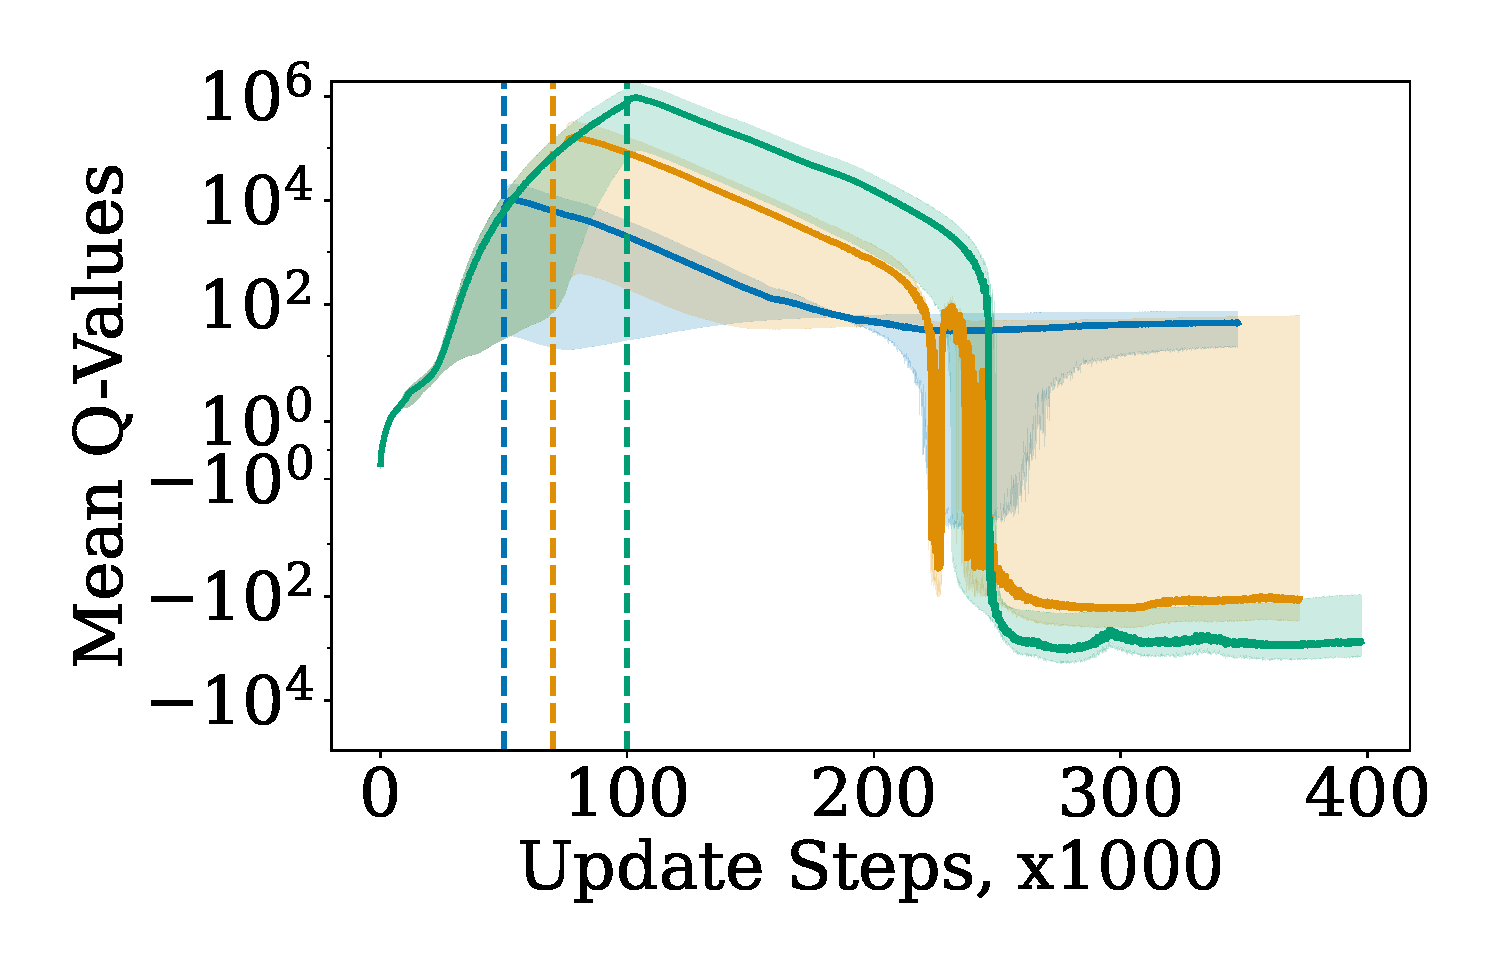
\includegraphics[width=4.7cm, trim=1cm 1cm 1cm 1cm ,clip]{figures/dissecting/priming/elu_priming_base_Q.pdf}
        \label{subfig:priming_base_Q}
    \end{subfigure}%
    \begin{subfigure}[b]{0.33\textwidth}
        \centering
        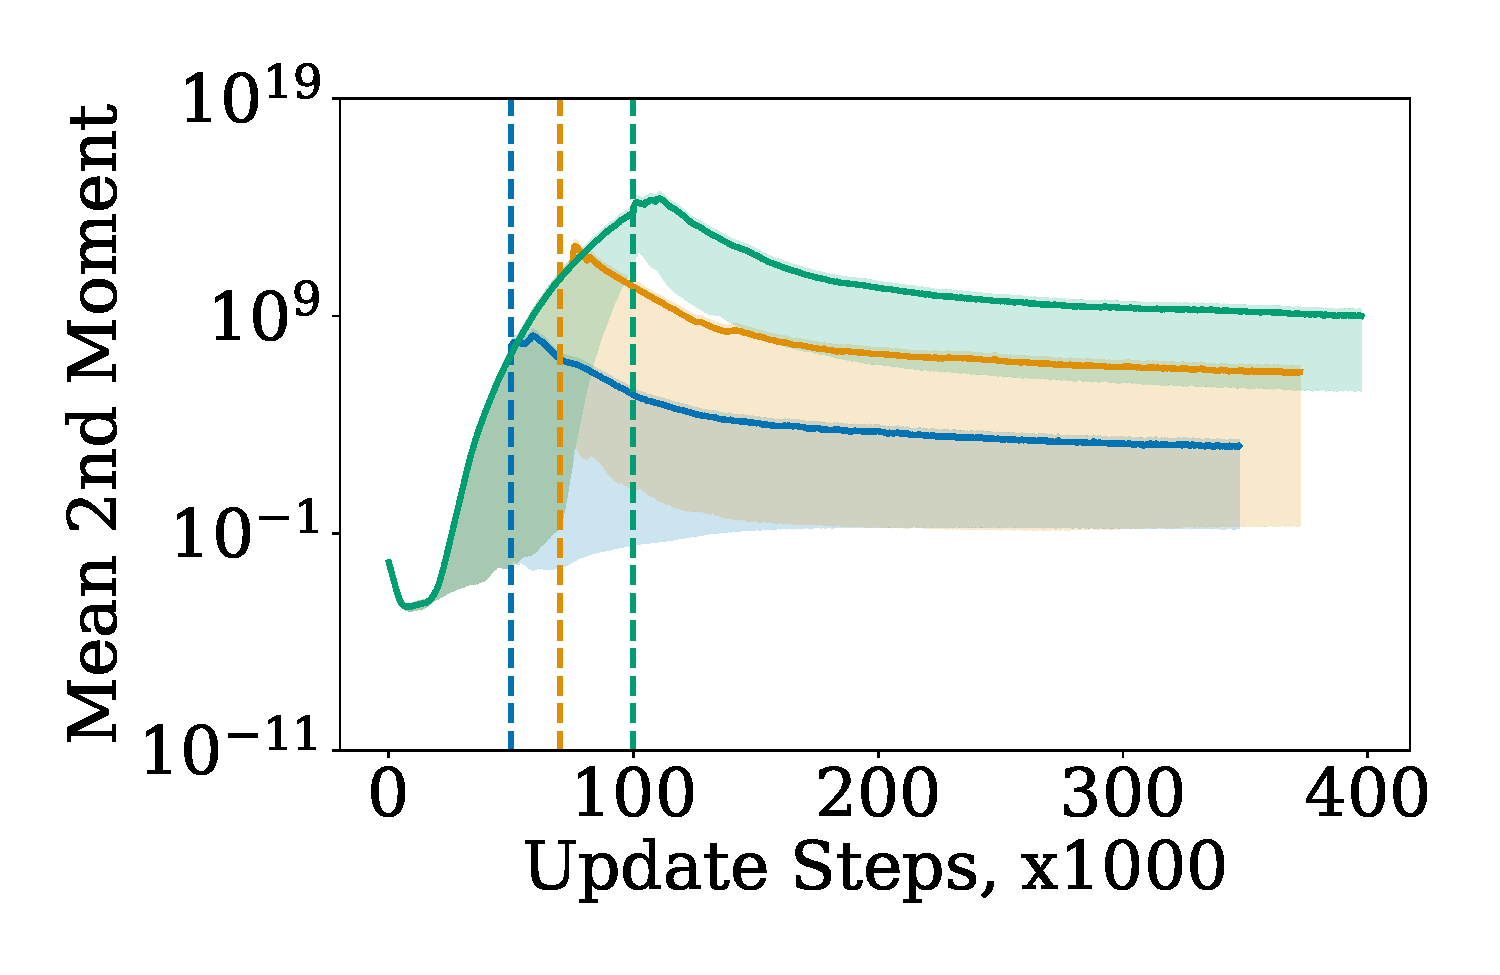
\includegraphics[width=4.7cm, trim=1cm 1cm 1cm 1cm ,clip]{figures/dissecting/priming/elu_priming_base_exp_avg_sq.pdf}
        \label{subfig:elu_priming_base_mom}
    \end{subfigure}%
    \vspace{-5pt}
    \caption{ELU activations. Return, in-distribution Q-values and Adam optimizer moments during priming for different lengths. Dotted lines correspond to end of priming. More priming leads to lower return and larger Q-value and optimizer divergence.}
    % \caption{Mean return, Q-values and Adam moments for priming of different lengths. Dotted lines indicate end of priming. More priming leads to lower return and Q-value and optimizer divergence.}
    \label{fig:elu_priming_base}
\end{figure}

During our experiments, we found that the ReLU activation can sometimes lead to destabilization of other parts of the SAC agent during priming. We found that using ELU~\parencite{clevert2016accurate} activations instead remedies some of these issues. We repeat various experiments from Section~\ref{sec:overestimation:investigating} again but with more stable activations. First, we show in Figure~\ref{fig:elu_priming_base} that divergence happens similar to before and that it is correlated with the amount of priming.

Furthermore, we discussed that the divergence is most likely triggered by out of distribution action prediction (see Figure~\ref{fig:overestimation:elu_priming_causes}) and that regularization can help. 
When using ELUs, the effect of regularization is much more stable and as expected but still not as good as our OFN approach from Section~\ref{sec:overestimation:evalmethod} (compare with Figure~\ref{fig:overestimation:elu_priming_abl}). 
Dropout leads to significantly worse performance and L$^2$ regularization learns Q-values too small for the obtained return which we suspect correlates with decreased exploration.

\begin{figure}[H]
\begin{minipage}[b]{.35\textwidth}
% \captionsetup[subfigure]{font=footnotesize, aboveskip=2pt}
\centering
    \begin{subfigure}[b]{\textwidth}
        \centering
        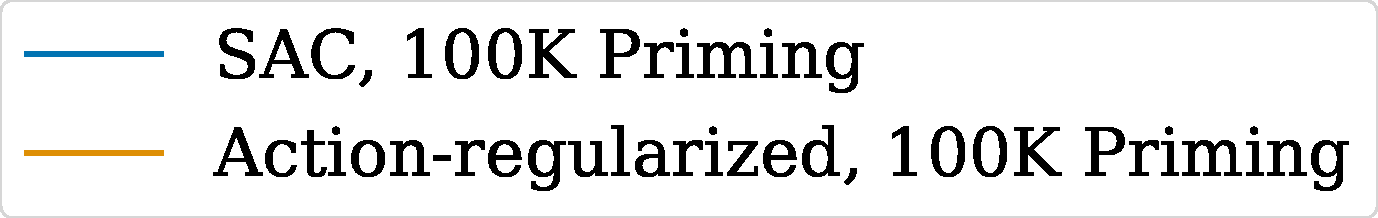
\includegraphics[height=0.8cm]{figures/dissecting/priming/elu_priming_causes_return_legend.pdf}
    \end{subfigure}\\%
    \begin{subfigure}[b]{\textwidth}
        \centering
        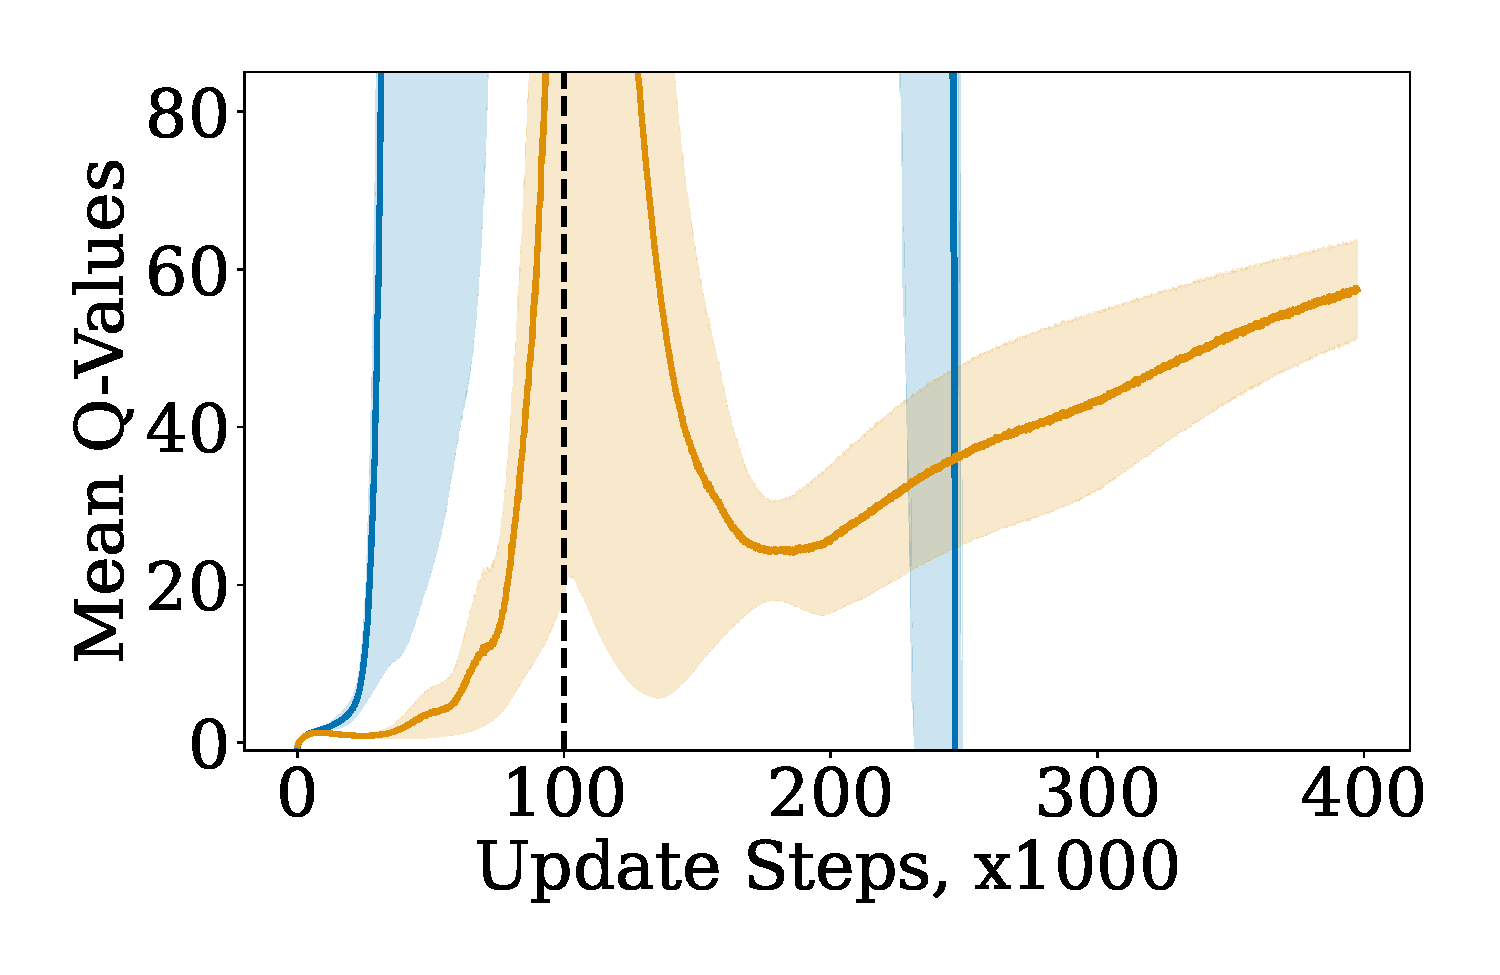
\includegraphics[width=4.8cm, trim=1cm 1cm 1cm 1cm ,clip]{figures/dissecting/priming/elu_priming_causes_Q.pdf}
        \label{subfig:elu_priming_causes_Q}
    \end{subfigure}%
    \vspace{-5pt}
    \caption{ELU activations. Priming with SAC and action regularization during priming. The latter lowers divergence. }
    \label{fig:elu_priming_causes}
\end{minipage}
\hfill
\begin{minipage}[b]{.62\textwidth}
% \captionsetup[subfigure]{font=footnotesize, aboveskip=2pt}
    \centering
    \begin{subfigure}[b]{0.8\textwidth}
        \centering
        
\includegraphics[height=0.4cm]{figures/dissecting/priming/elu_priming_ablations_return_legend.pdf}
    \end{subfigure}\\%
    \begin{subfigure}[b]{0.5\textwidth}
        \centering
        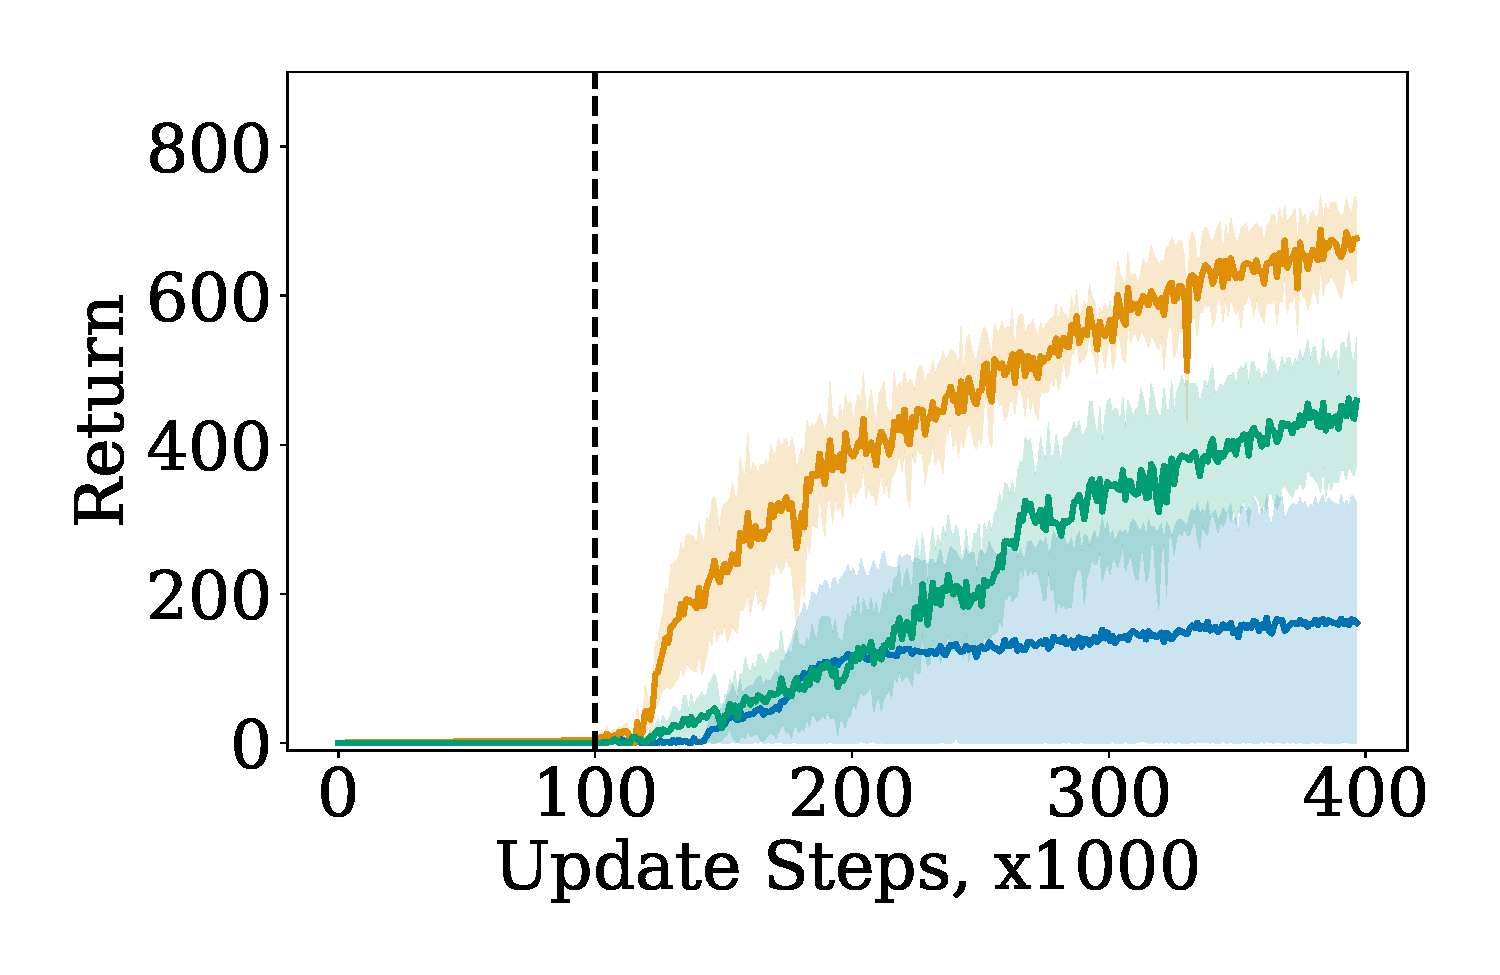
\includegraphics[width=4.8cm, trim=1cm 1cm 1cm 1cm ,clip]{figures/dissecting/priming/elu_priming_ablations_return.pdf}
        \label{subfig:elu_priming_abl_ret}
    \end{subfigure}%
    \begin{subfigure}[b]{0.5\textwidth}
    \centering
        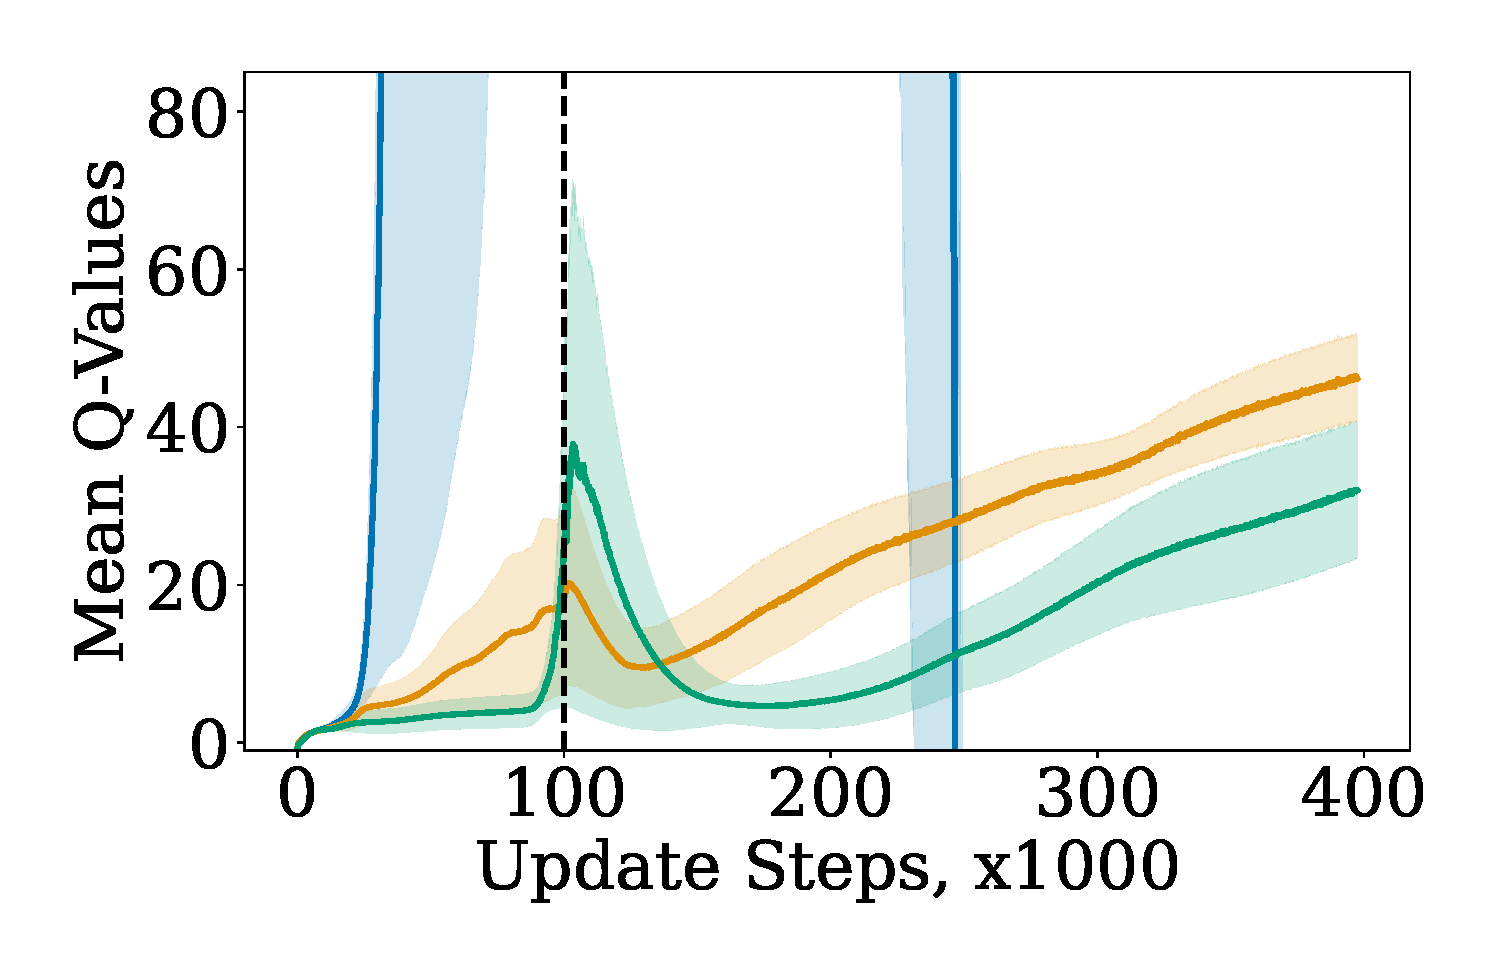
\includegraphics[width=4.8cm, trim=1cm 1cm 1cm 1cm ,clip]{figures/dissecting/priming/elu_priming_ablations_Q.pdf}
        \label{subfig:elu_priming_abl_Q}
    \end{subfigure}%
    \vspace{-18pt}
    \caption{ELU activations. Return and
    Q-values of priming runs with weight decay and dropout. Results indicate that both regularizations mitigate priming more than with ReLUs. }
    \label{fig:elu_priming_abl}
\end{minipage}
    \vspace{-5pt}
\end{figure}

\subsection{Optimizer divergence} \label{app:priming_opt}

With more stable effects from the ELU activation, we introduce a second intervention to the priming stage. We hypothesize that most of the divergence stems from the second optimizer term that will propell the gradients to increase more and more over time. To test this, we run an additional experiment in which we use standard stochastic gradient descent (SGD)~\parencite{robbins1951stochastic} with first-order momentum~\parencite{rumelhart1986learning, sutskever2013on} during priming to isolate the effect of the second-order momentum term. We compare this against RMSProp which is equivalent to Adam but without the first optimizer term instead. The results are shown in Figure~\ref{app:priming_opt}. As we can see, the divergence is almost completely gone when using SGD with momentum but is even larger in RMSProp. Note that running the same experiment with ReLU activations  leads to divergence in the actor when using SGD only. We suspect this might have to do with divergence in the actor entropy.

\begin{figure}[H]
% \captionsetup[subfigure]{font=footnotesize, aboveskip=2pt}
\centering
    \begin{subfigure}[b]{0.8\textwidth}
        \centering
        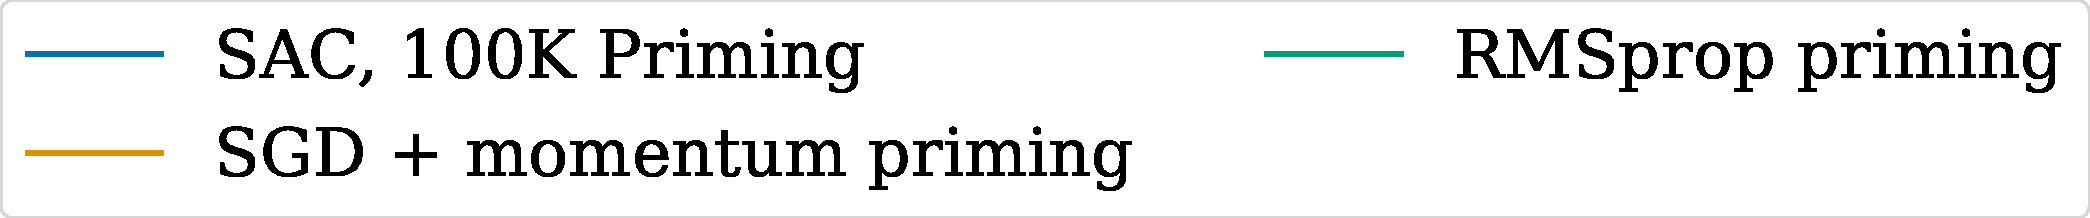
\includegraphics[height=0.8cm]{figures/dissecting/priming/elu_priming_opt_return_legend.pdf}
    \end{subfigure}\\%
    \begin{subfigure}[b]{0.33\textwidth}
        \centering
        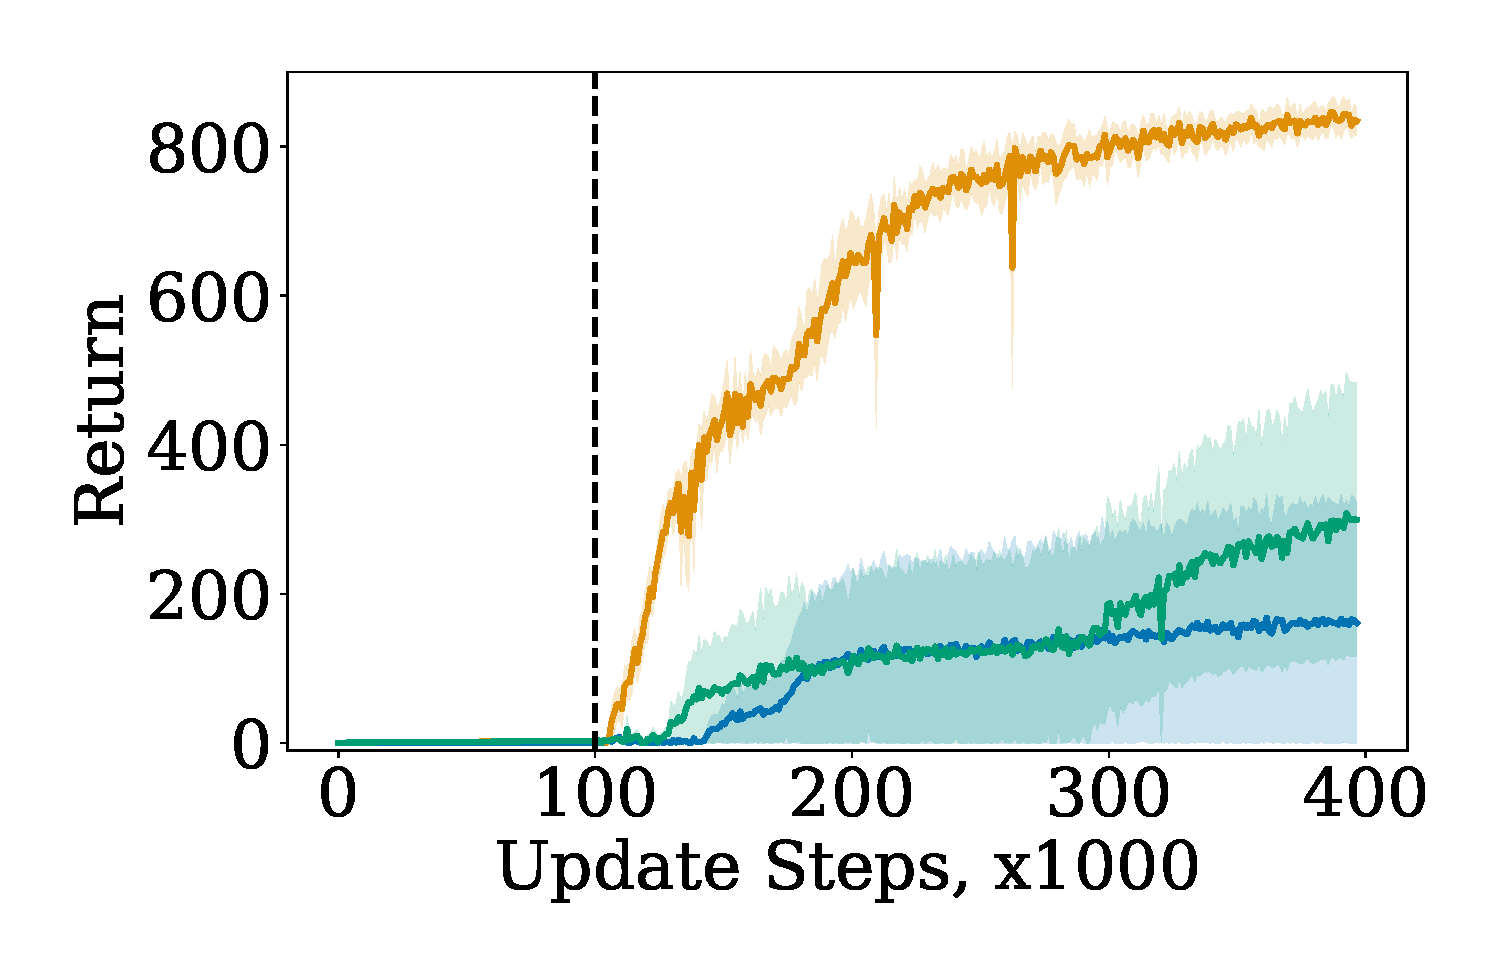
\includegraphics[width=4.7cm, trim=1cm 1cm 1cm 1cm ,clip]{figures/dissecting/priming/elu_priming_opt_return.pdf}
        \label{subfig:priming_opt_ret}
    \end{subfigure}%
    \begin{subfigure}[b]{0.33\textwidth}
    \centering
        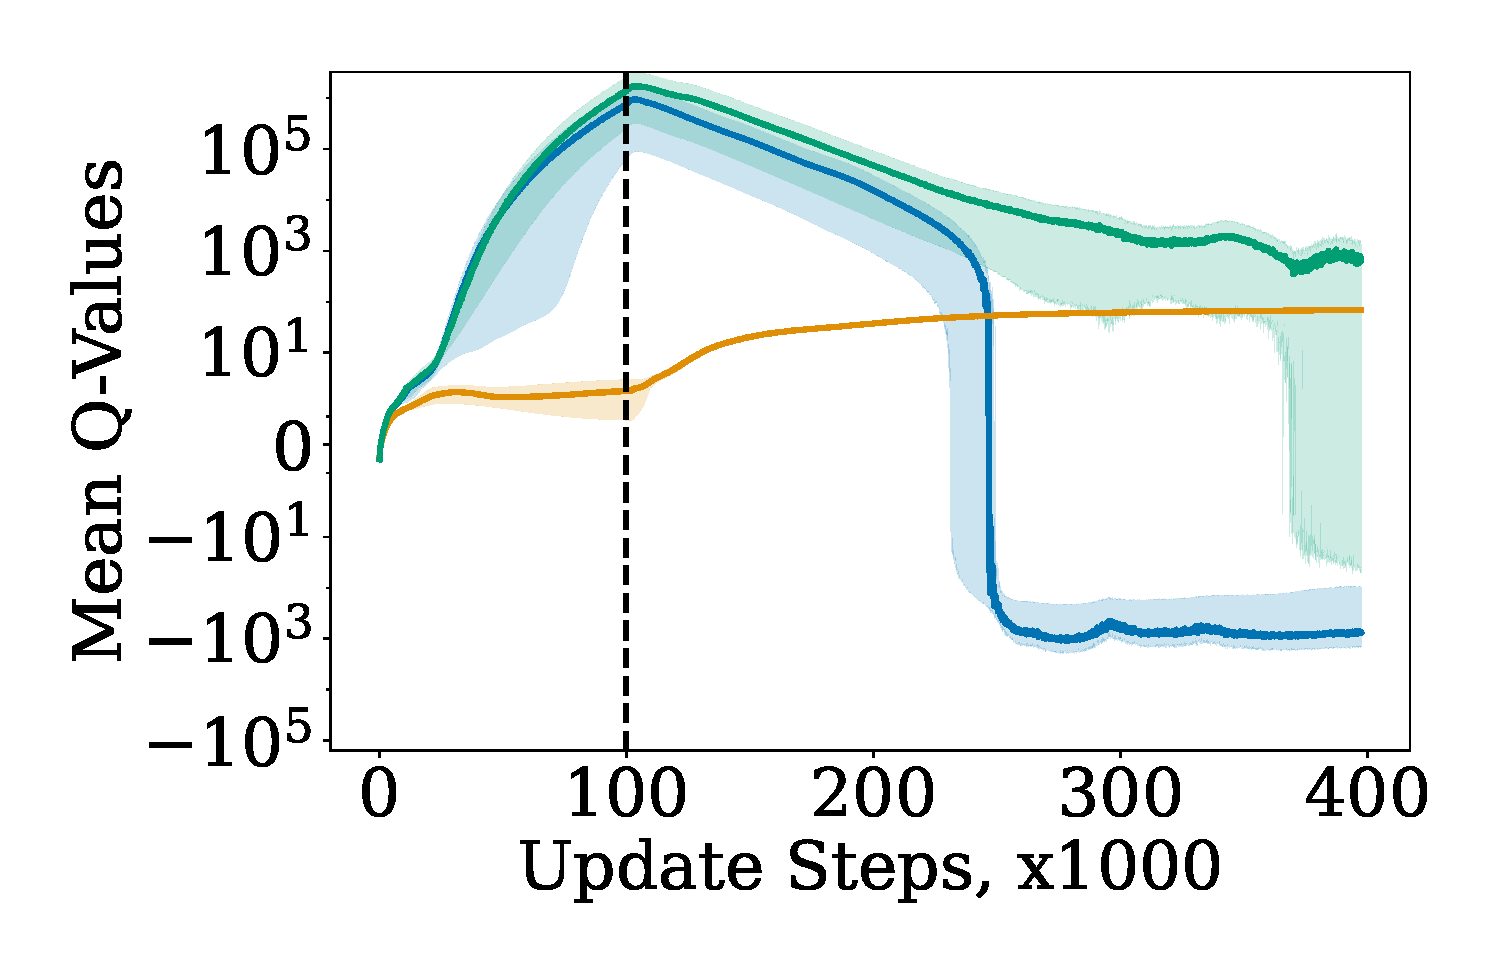
\includegraphics[width=4.7cm, trim=1cm 1cm 1cm 1cm ,clip]{figures/dissecting/priming/elu_priming_opt_Q.pdf}
        \label{subfig:priming_opt_Q}
    \end{subfigure}%
    \vspace{-5pt}
    \caption{Comparing standard SAC priming to priming when using either SGD+momentum or RMSProp during the priming updates. SGD+momentum does not diverge with ELU activations, indicating that the second-order momentum term is the problematic one.}
    \label{fig:priming_opt}
\end{figure}

\subsection{Effective dimension} \label{app:priming_dim}

Let $\Phi \in \mathbb{R}^{|\mathcal{S}| |\mathcal{A}| \times d}$ be a feature matrix (in our case produced by $\phi$). The effective dimension of a feature matrix has previously been defined as 
\begin{equation*}
    \text{srank}_{\delta} = \min 
    \left\{ k : \cfrac{\sum_{i=1}^k \sigma_i(\Phi)}{\sum_{i=1}^d \sigma_i(\Phi) \geq 1 - \delta}
    \right\} \enspace ,
\end{equation*}
where $\delta$ is a threshold parameters and $\{\sigma_i(\Phi)\}$ are the singular values of $\Phi$ in decreasing order~\parencite{yang2020harnessing, kumar2021implicit}.

An additional finding of ours is that divergence of Q-values is correlated with this effective rank $\text{srank}_{\delta}$. We plot three different random seeds that have been subjected to 75,000 steps of priming in Figure~\ref{fig:elu_priming_dim}; the effective rank is approximated over a sample 10 times the size of the embedding dimension. We observe, that divergence correlates with a decrease in effective dimension and that when divergence is exceptionally strong, the effective dimension drops so low that the agent has trouble to continue learning. This might explain the failure to learn observed by~\textcite{nikishin2022primacy}. However, as long as the effective dimension does not drop too far, the agent can recover and regain capacity by observing new data. 
Previous work on effective rank loss has often assumed that it is mostly irreversible, yet we find that this is not always the case.
We suspect that in complete failure cases, the policy has collapse and rarely any new data is seen.

\begin{figure}[H]
% \captionsetup[subfigure]{font=footnotesize, aboveskip=2pt}
\centering
    \begin{subfigure}[b]{0.8\textwidth}
        \centering
        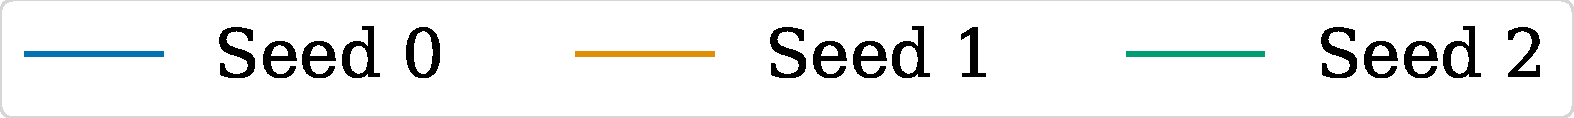
\includegraphics[height=0.4cm]{figures/dissecting/priming/elu_dim_return_legend.pdf}
    \end{subfigure}\\%
    \begin{subfigure}[b]{0.33\textwidth}
        \centering
        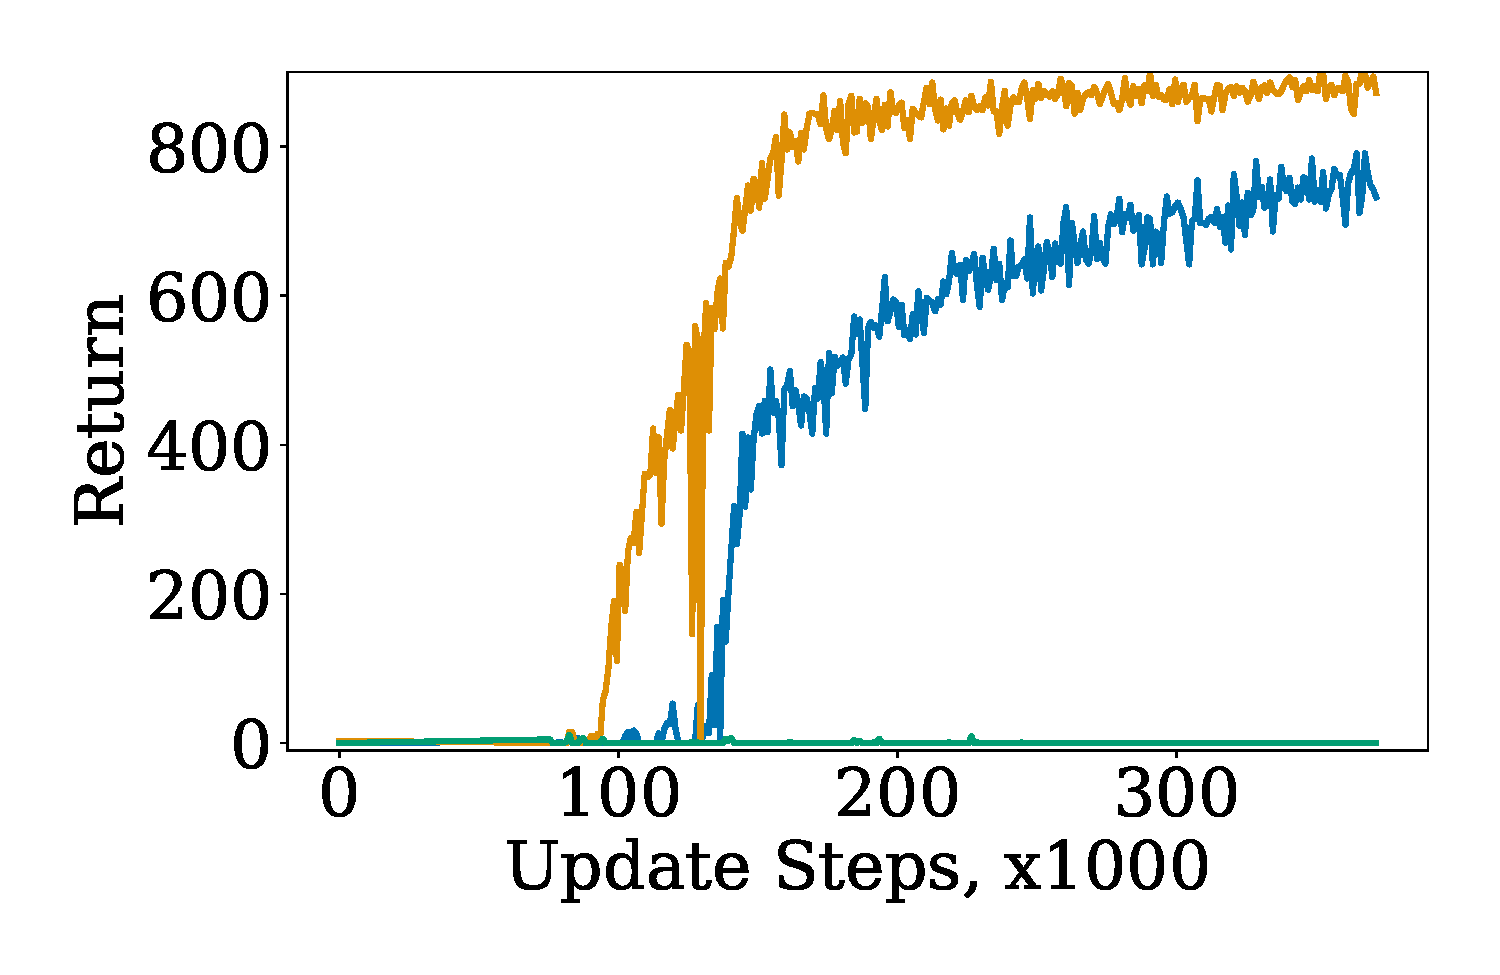
\includegraphics[width=4.7cm, trim=1cm 1cm 1cm 1cm ,clip]{figures/dissecting/priming/elu_dim_return.pdf}
        \label{subfig:elu_dim_ret}
    \end{subfigure}%
    \begin{subfigure}[b]{0.33\textwidth}
    \centering
        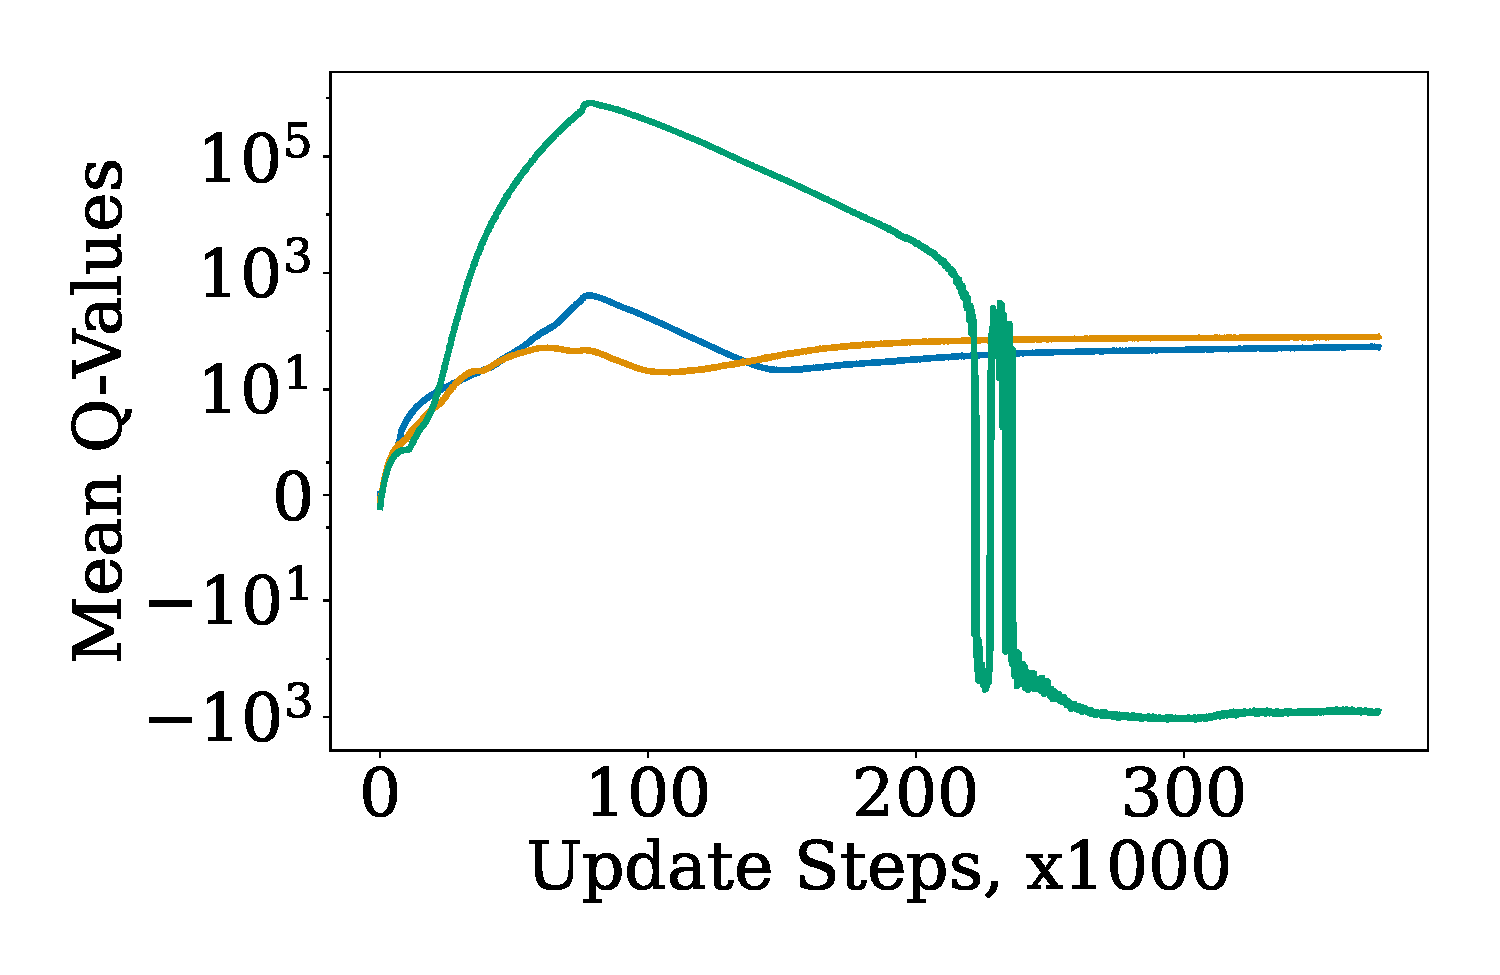
\includegraphics[width=4.7cm, trim=1cm 1cm 1cm 1cm ,clip]{figures/dissecting/priming/elu_dim_Q.pdf}
        \label{subfig:priming_dim_Q}
    \end{subfigure}%
    \begin{subfigure}[b]{0.33\textwidth}
        \centering
        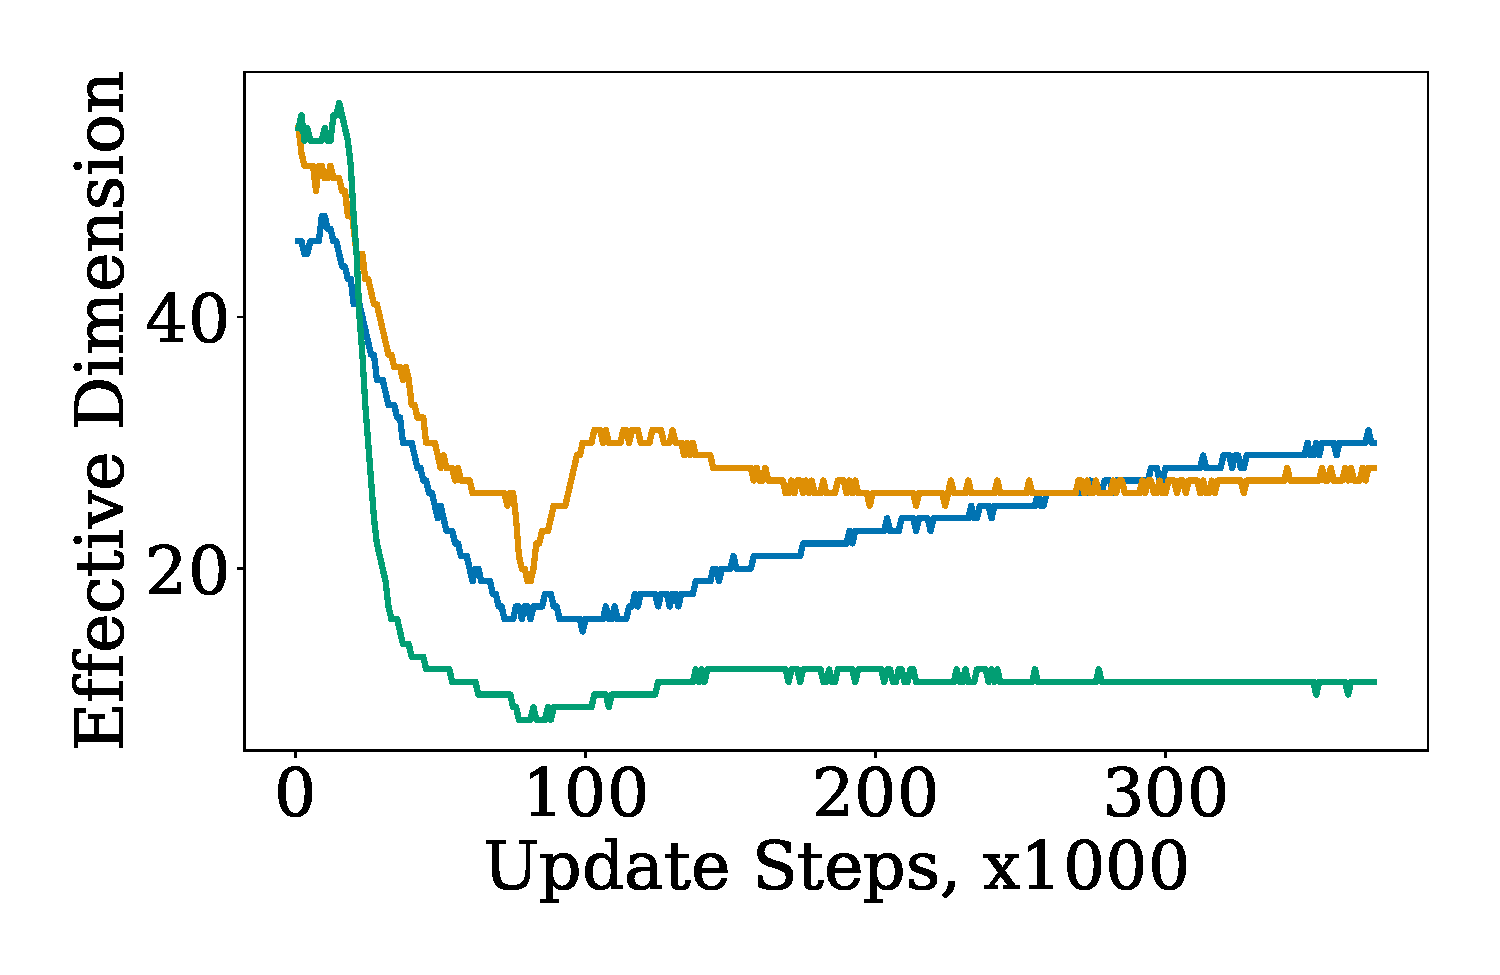
\includegraphics[width=4.7cm, trim=1cm 1cm 1cm 1cm ,clip]{figures/dissecting/priming/elu_dim_ed.pdf}
        \label{subfig:elu_priming_dim_ed}
    \end{subfigure}%
    \vspace{-5pt}
    \caption{Returns, Mean Q-values and effective dimension for $3$ seeds of standard priming for 75,000 steps. When divergence happens, effective dimension is lost. If the effective dimension drops too far, the agent has difficulties to recover.}
    % \caption{Mean return, Q-values and Adam moments for priming of different lengths. Dotted lines indicate end of priming. More priming leads to lower return and Q-value and optimizer divergence.}
    \label{fig:elu_priming_dim}
\end{figure}

\newpage

\section{Additional experimental results} \label{app:exp}

\subsection{Returns on all environments} \label{app:exp_ret}

\begin{figure}[H]
% \captionsetup[subfigure]{font=footnotesize, aboveskip=2pt}
\centering
    \begin{subfigure}[b]{0.8\textwidth}
        \centering
        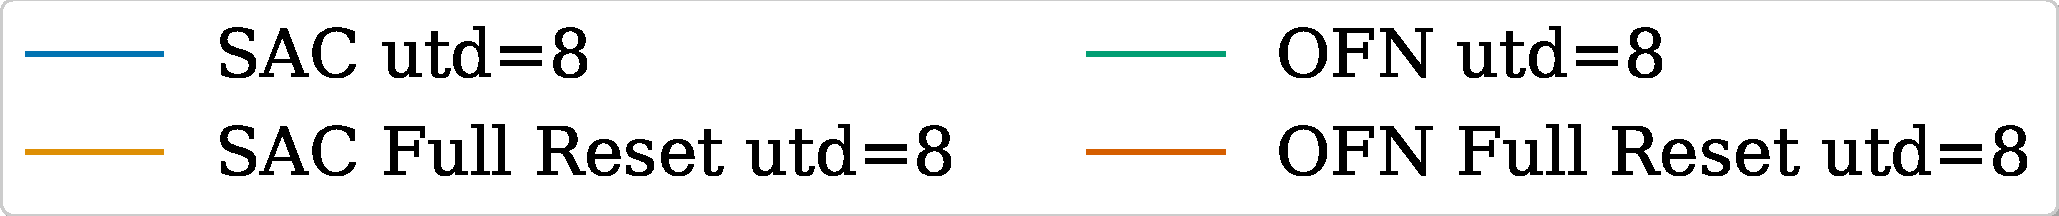
\includegraphics[height=0.8cm]{figures/dissecting/main_exp/utd_8_return_legend.pdf}
    \end{subfigure}\\%
    \begin{subfigure}[b]{1\textwidth}
        \centering
        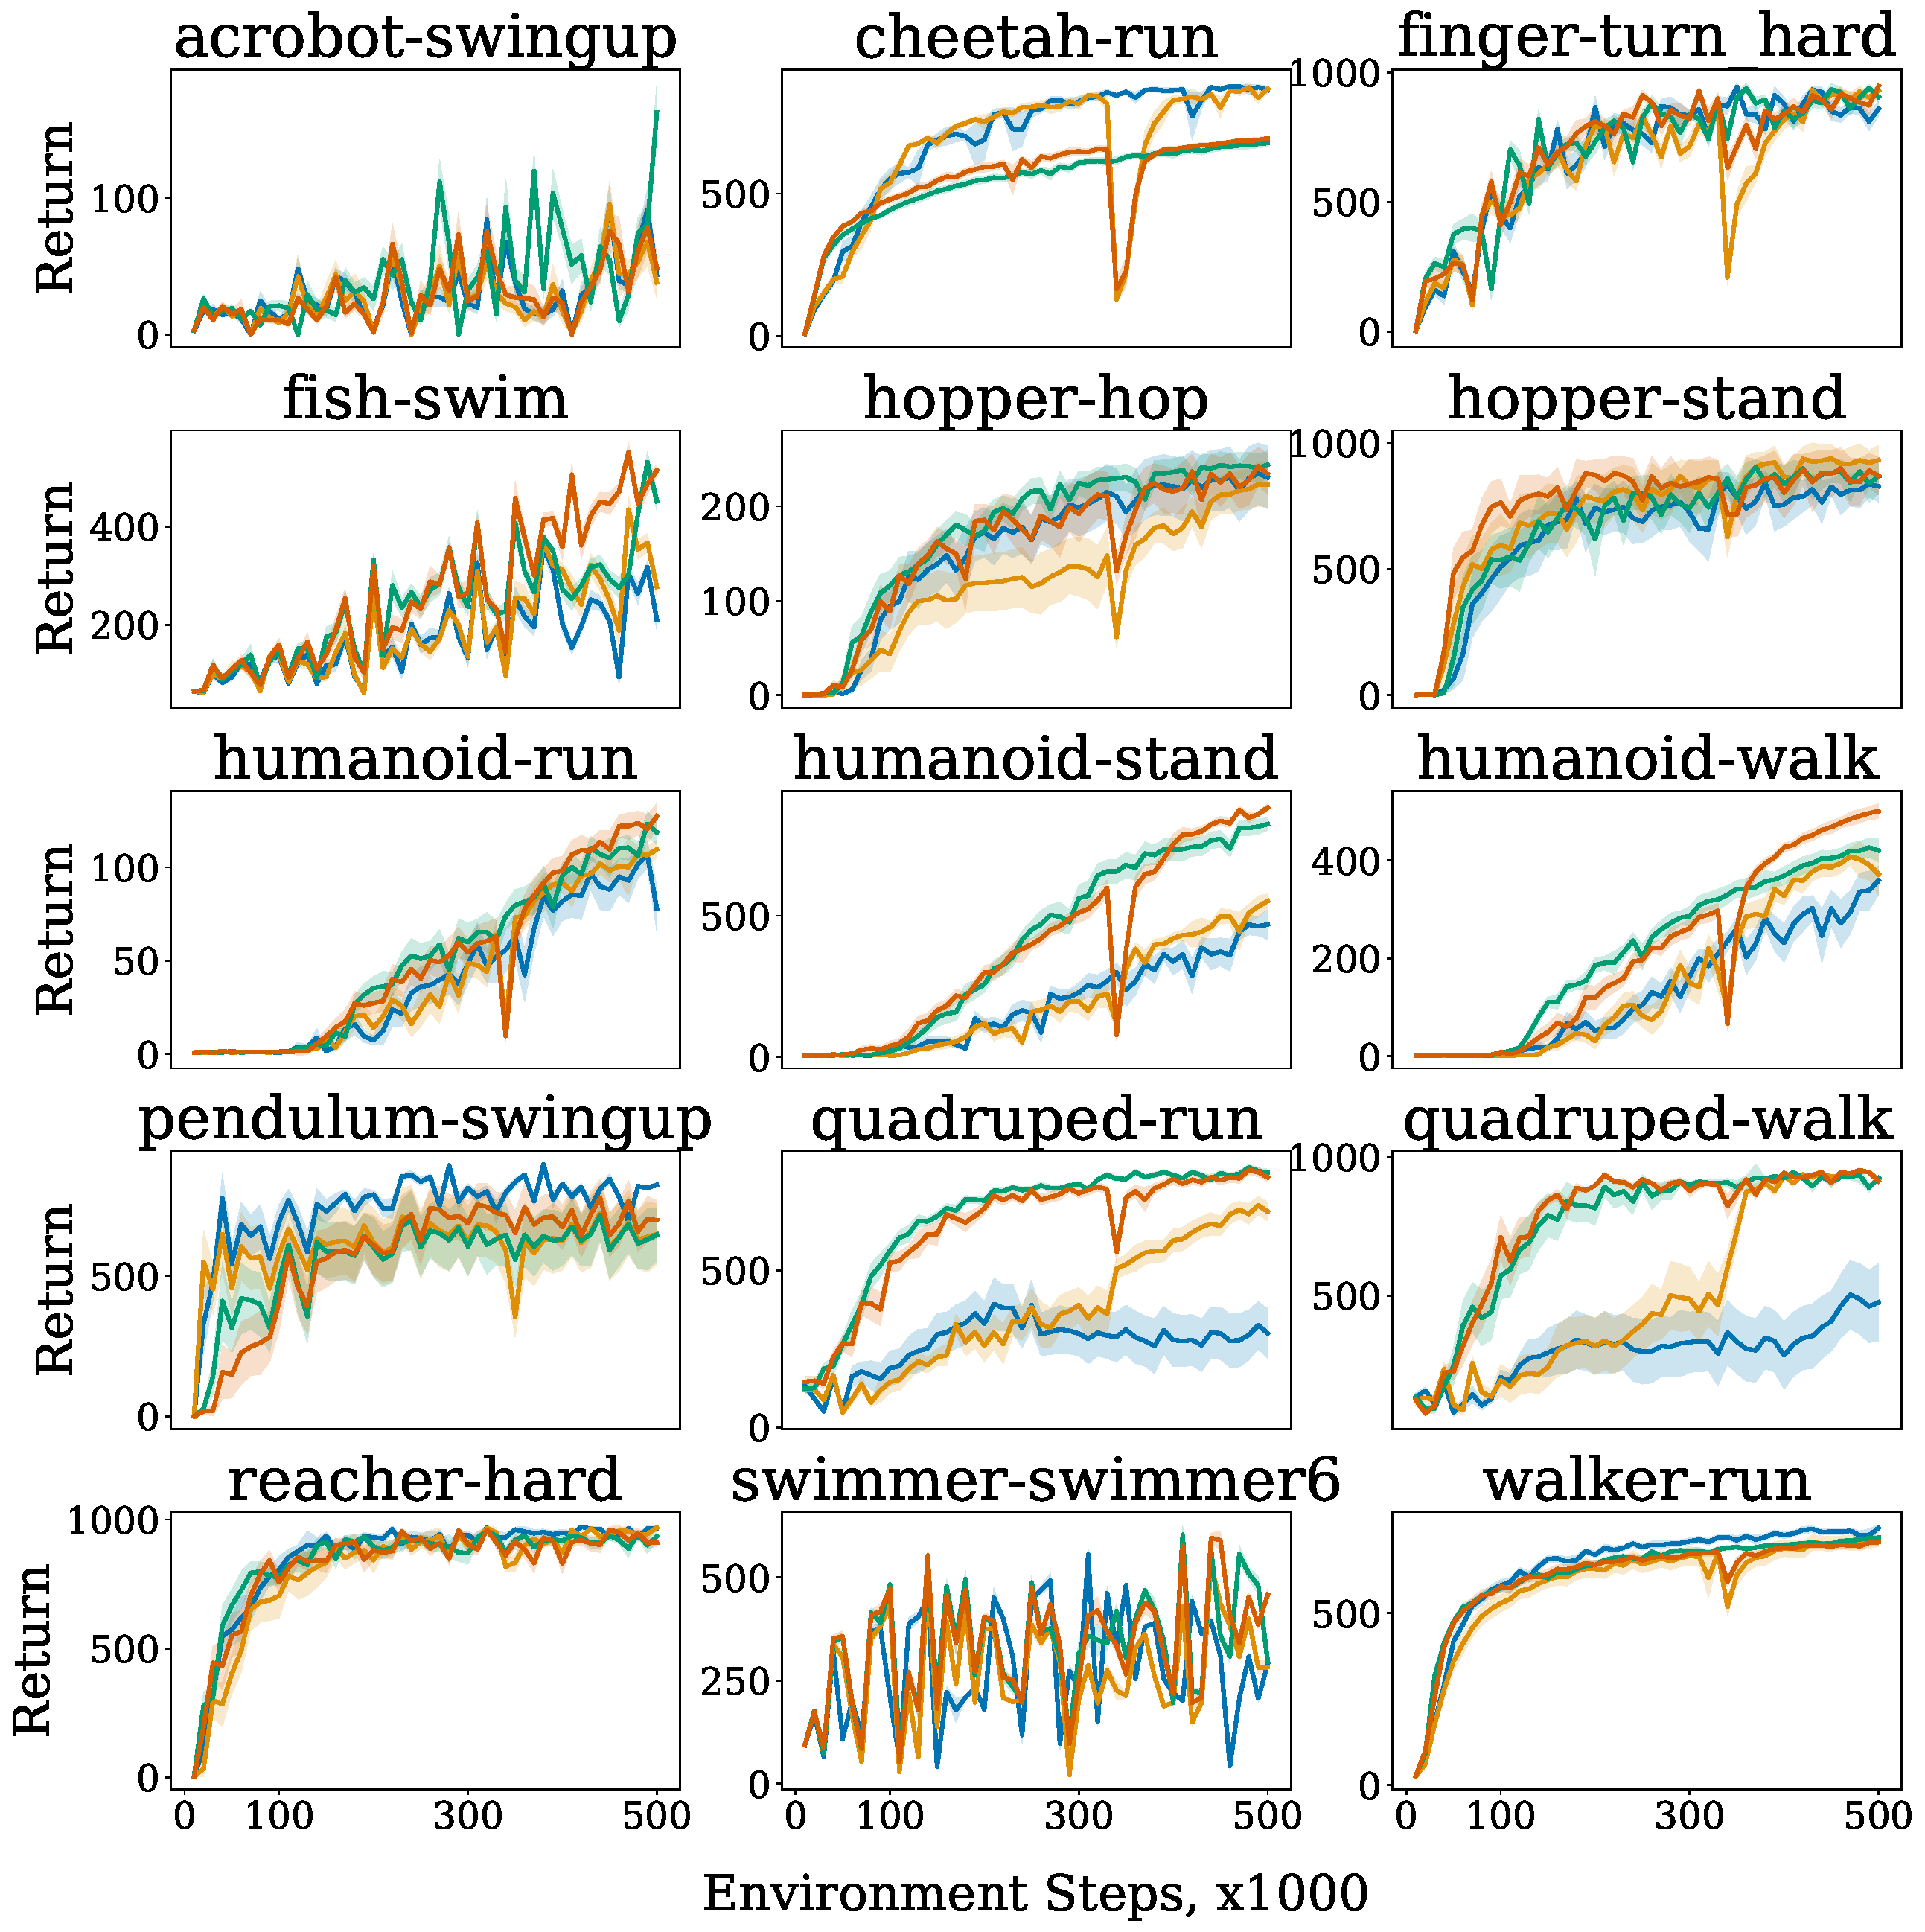
\includegraphics[width=15cm, trim=0cm 0cm 0cm 0cm ,clip]{figures/dissecting/main_exp/utd_8_return.pdf}
    \end{subfigure}%
    \vspace{-5pt}
    \caption{UTD8 Returns on Full DMC15-500K.}
    % \caption{Mean return, Q-values and Adam moments for priming of different lengths. Dotted lines indicate end of priming. More priming leads to lower return and Q-value and optimizer divergence.}
    \label{fig:utd8_ret}
\end{figure}

\newpage

\begin{figure}[H]
% \captionsetup[subfigure]{font=footnotesize, aboveskip=2pt}
\centering
    \begin{subfigure}[b]{0.8\textwidth}
        \centering
        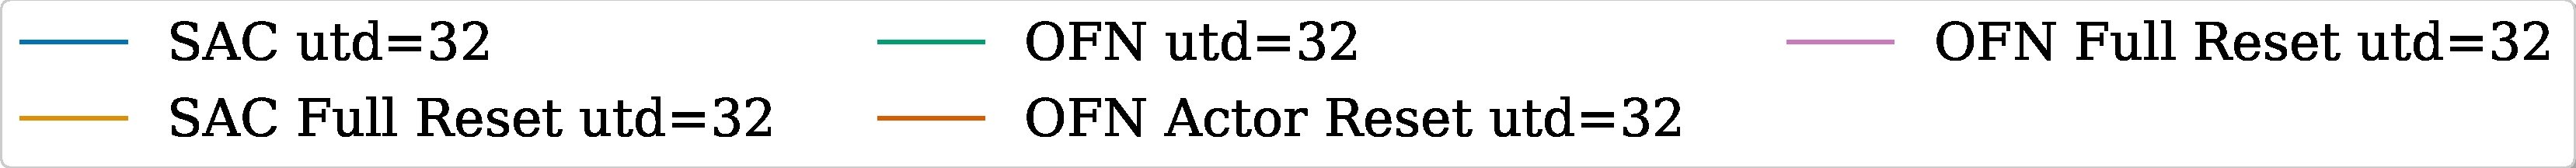
\includegraphics[height=0.8cm]{figures/dissecting/main_exp/utd_32_return_legend.pdf}
    \end{subfigure}\\%
    \begin{subfigure}[b]{1\textwidth}
        \centering
        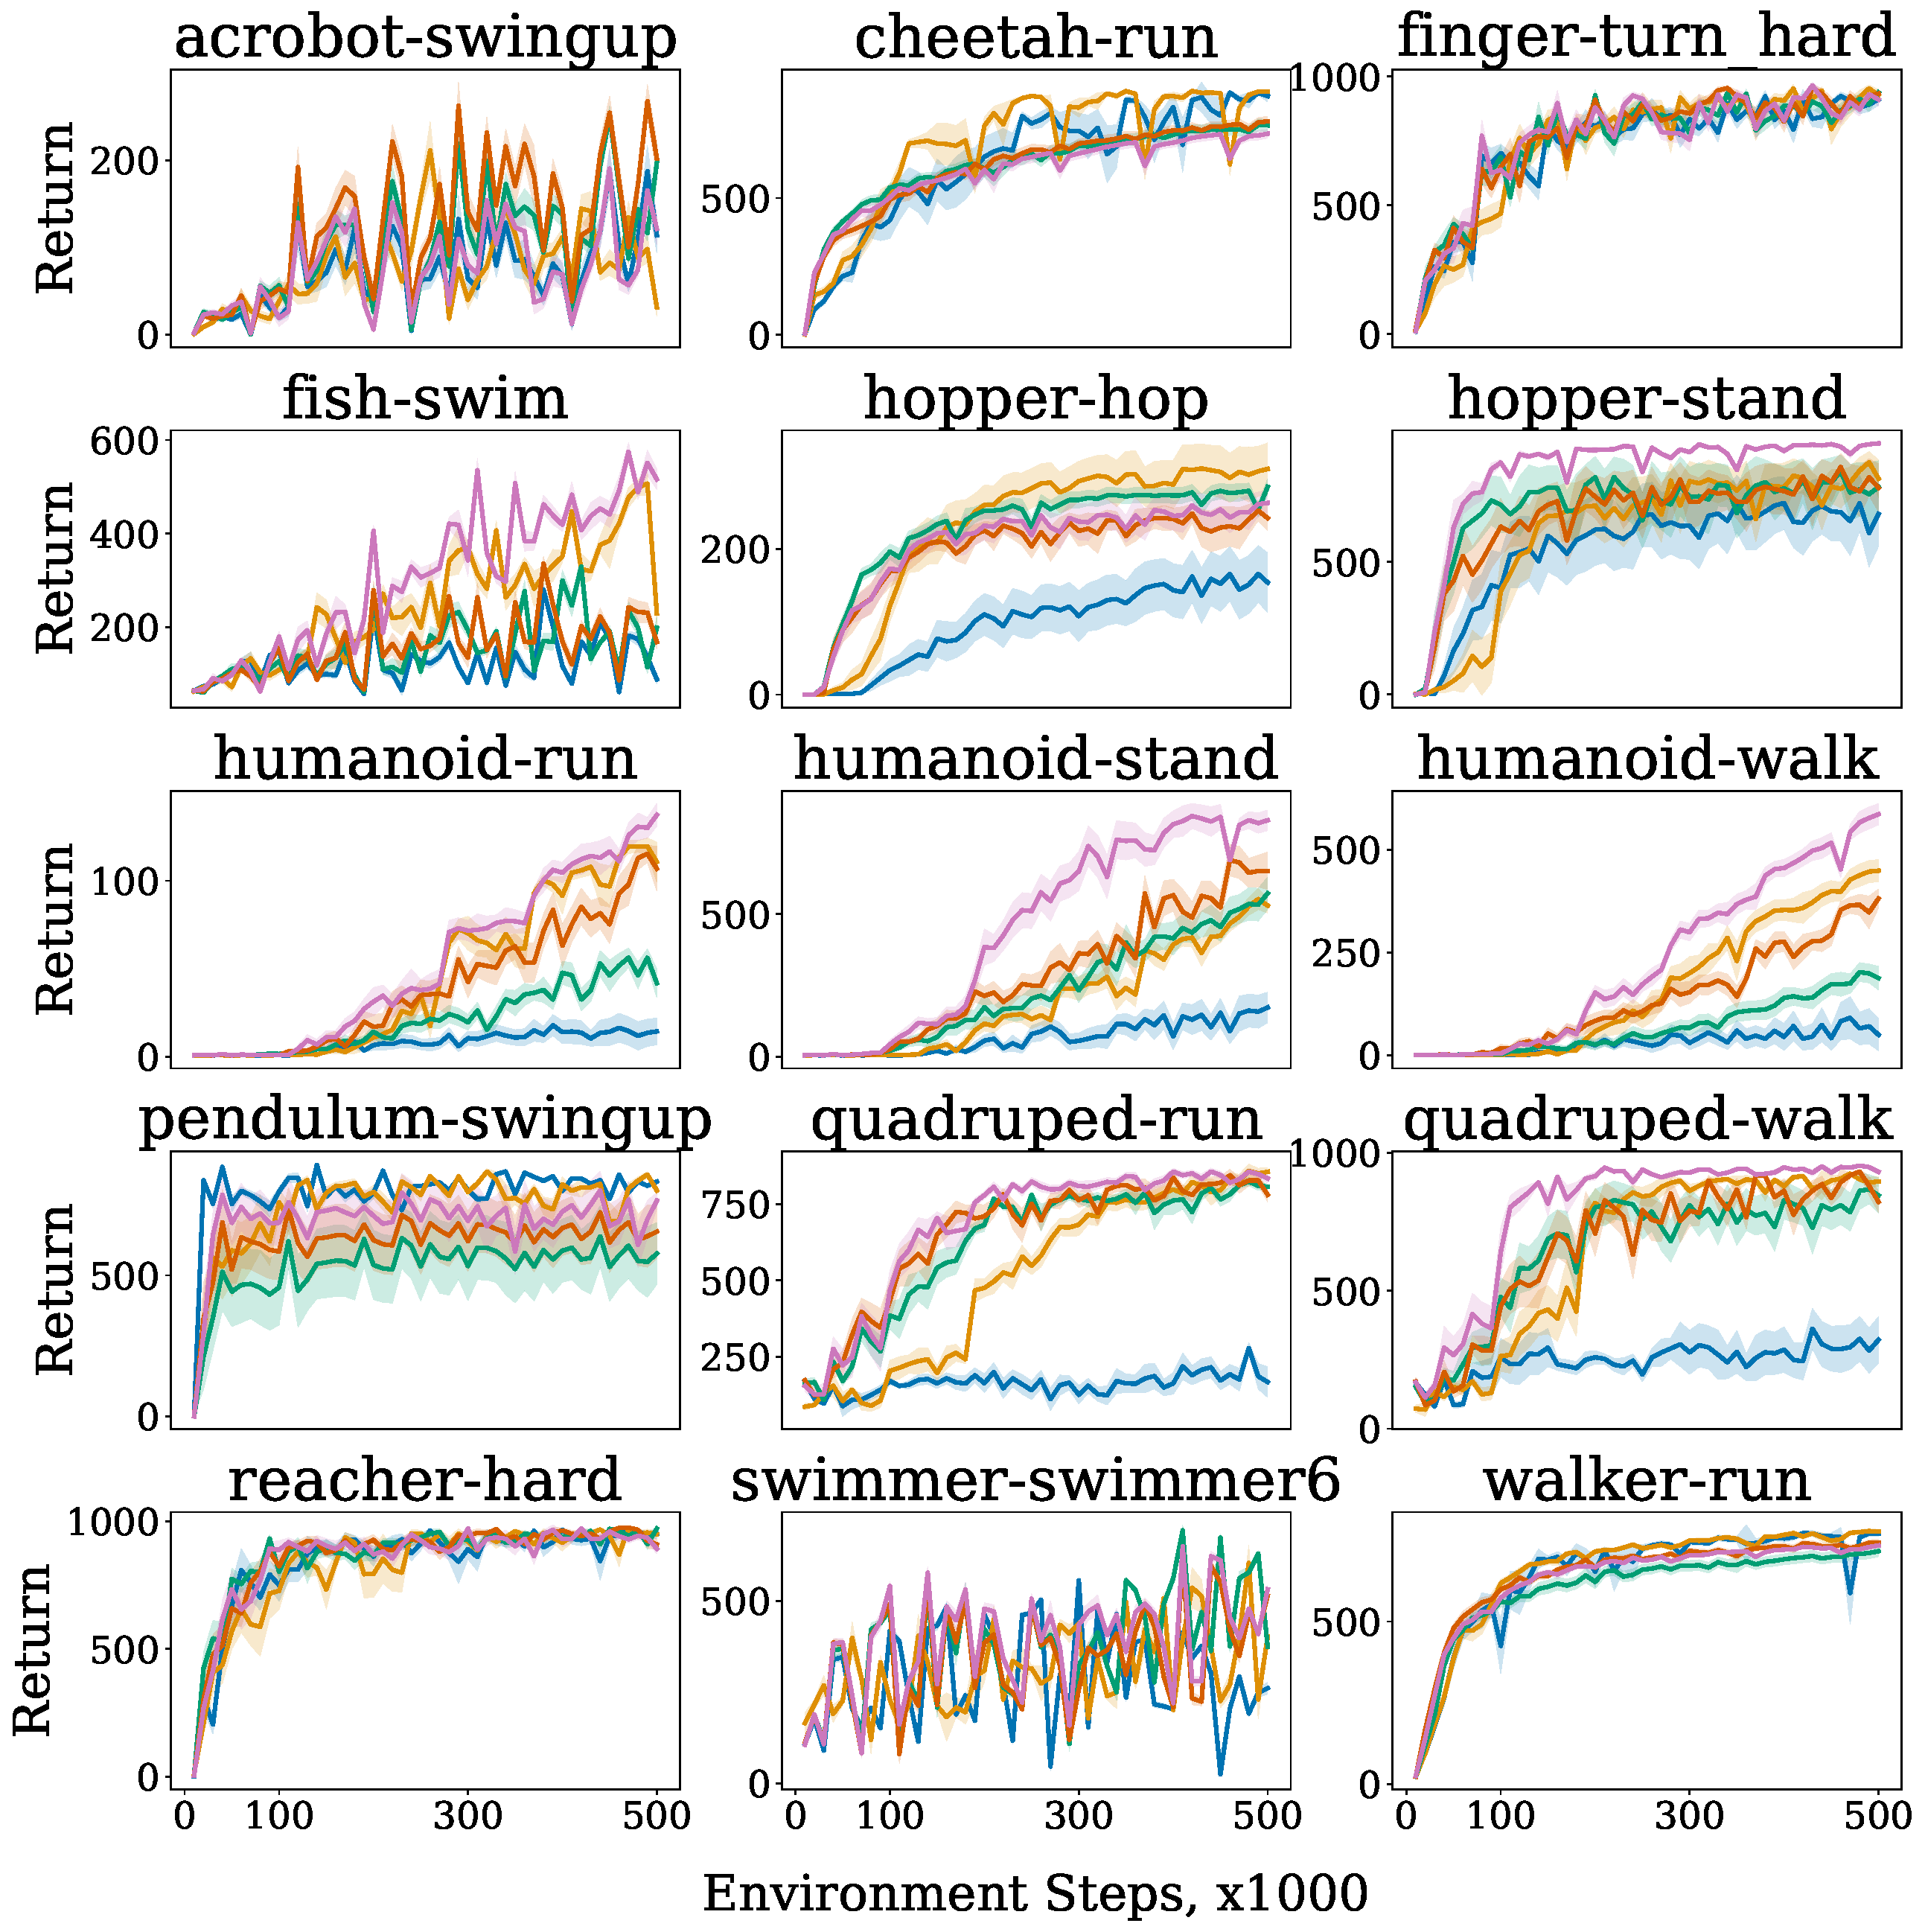
\includegraphics[width=15cm, trim=0cm 0cm 0cm 0cm ,clip]{figures/dissecting/main_exp/utd_32_return.pdf}
    \end{subfigure}%
    \vspace{-5pt}
    \caption{UTD32 Returns on Full DMC15-500K.}
    % \caption{Mean return, Q-values and Adam moments for priming of different lengths. Dotted lines indicate end of priming. More priming leads to lower return and Q-value and optimizer divergence.}
    \label{fig:utd32_ret}
\end{figure}

\newpage

\subsection{Q-values on all environments} \label{app:exp_q}

\begin{figure}[H]
% \captionsetup[subfigure]{font=footnotesize, aboveskip=2pt}
\centering
    \begin{subfigure}[b]{0.8\textwidth}
        \centering
        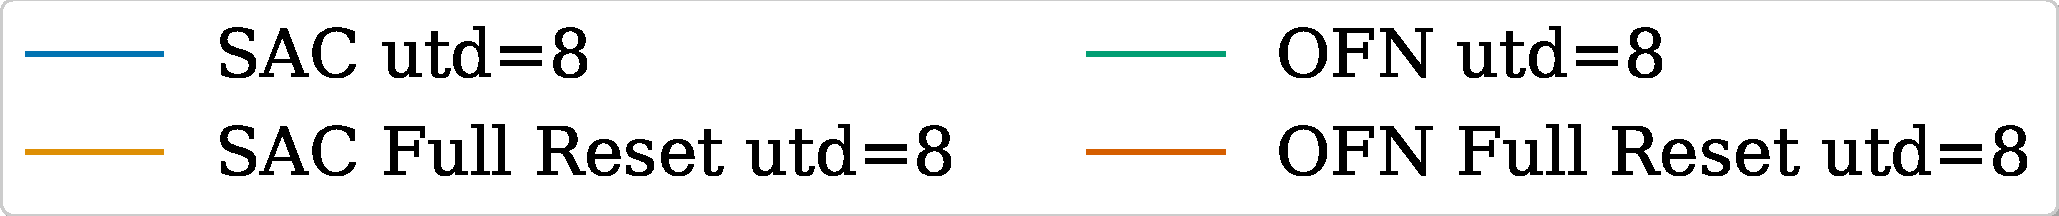
\includegraphics[height=0.8cm]{figures/dissecting/main_exp/utd_8_Q_legend.pdf}
    \end{subfigure}\\%
    \begin{subfigure}[b]{1\textwidth}
        \centering
        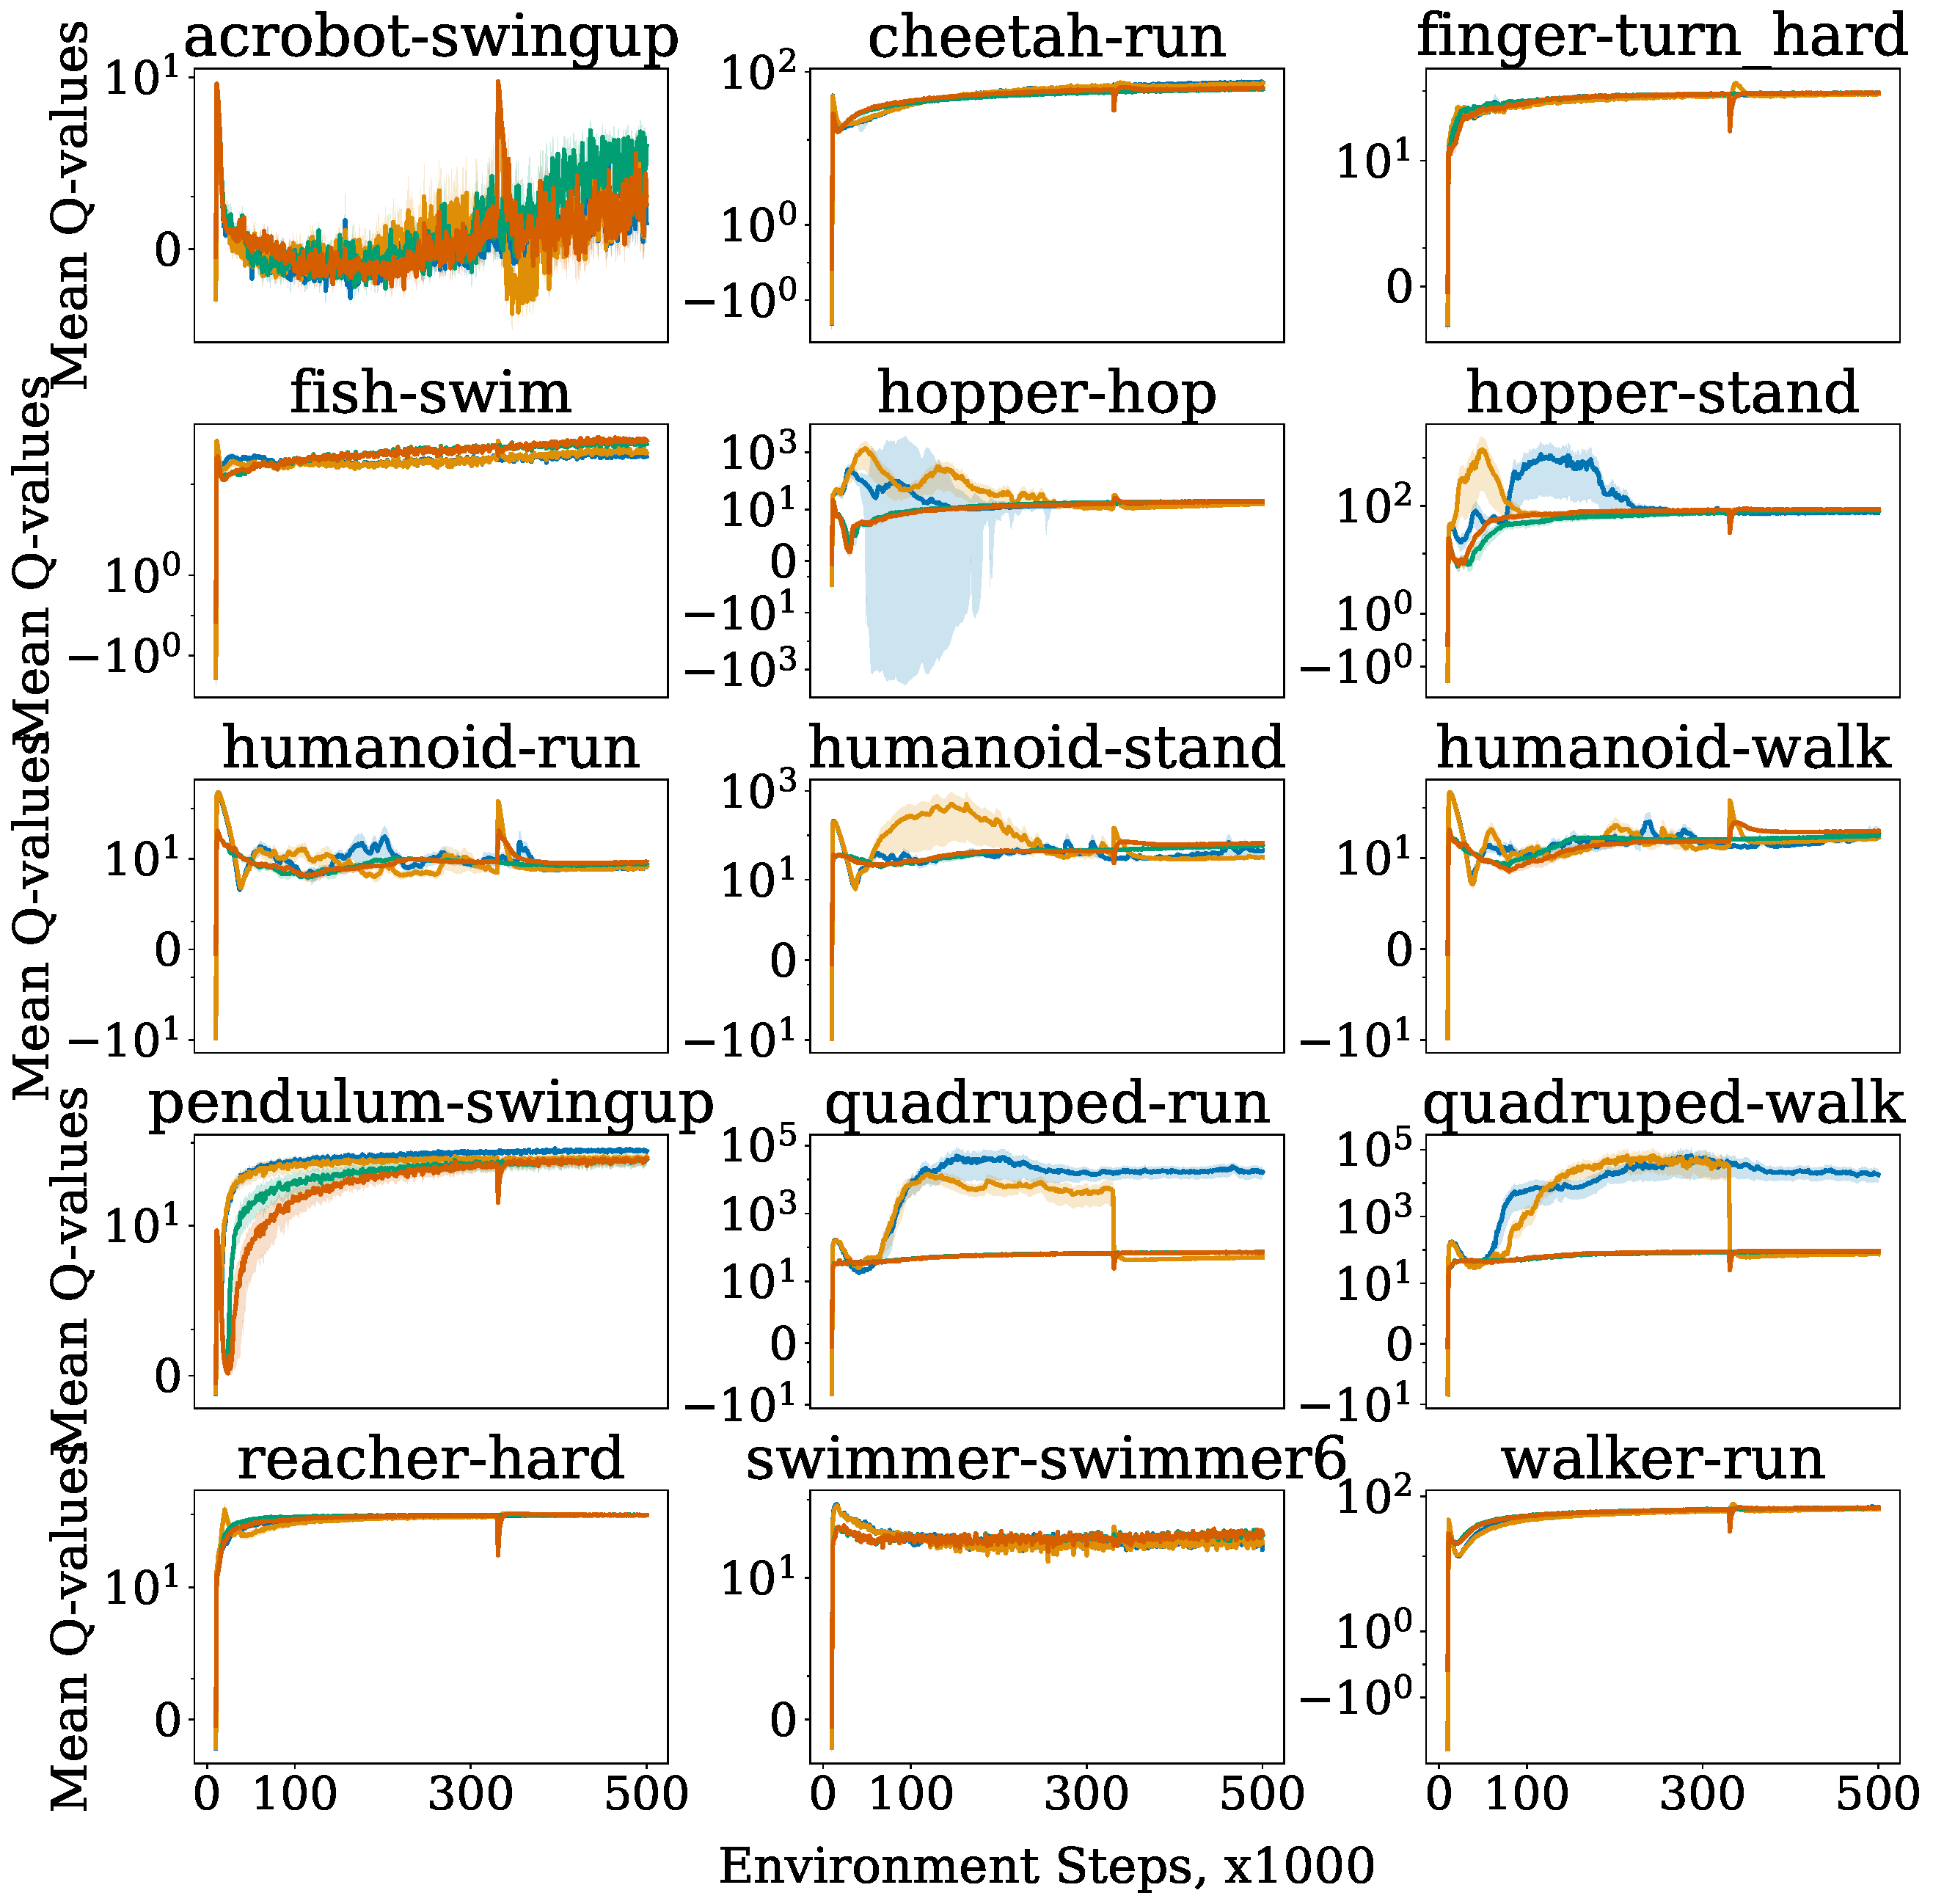
\includegraphics[width=15cm, trim=0cm 0cm 0cm 0cm ,clip]{figures/dissecting/main_exp/utd_8_Q.pdf}
    \end{subfigure}%
    \vspace{-5pt}
    \caption{UTD8 Q-values on Full DMC15-500K. Resetting often works when Q-values diverge. ONF mitigates divergence.}
    % \caption{Mean return, Q-values and Adam moments for priming of different lengths. Dotted lines indicate end of priming. More priming leads to lower return and Q-value and optimizer divergence.}
    \label{fig:utd8_Q}
\end{figure}

\newpage

\begin{figure}[H]
% \captionsetup[subfigure]{font=footnotesize, aboveskip=2pt}
\centering
    \begin{subfigure}[b]{0.8\textwidth}
        \centering
        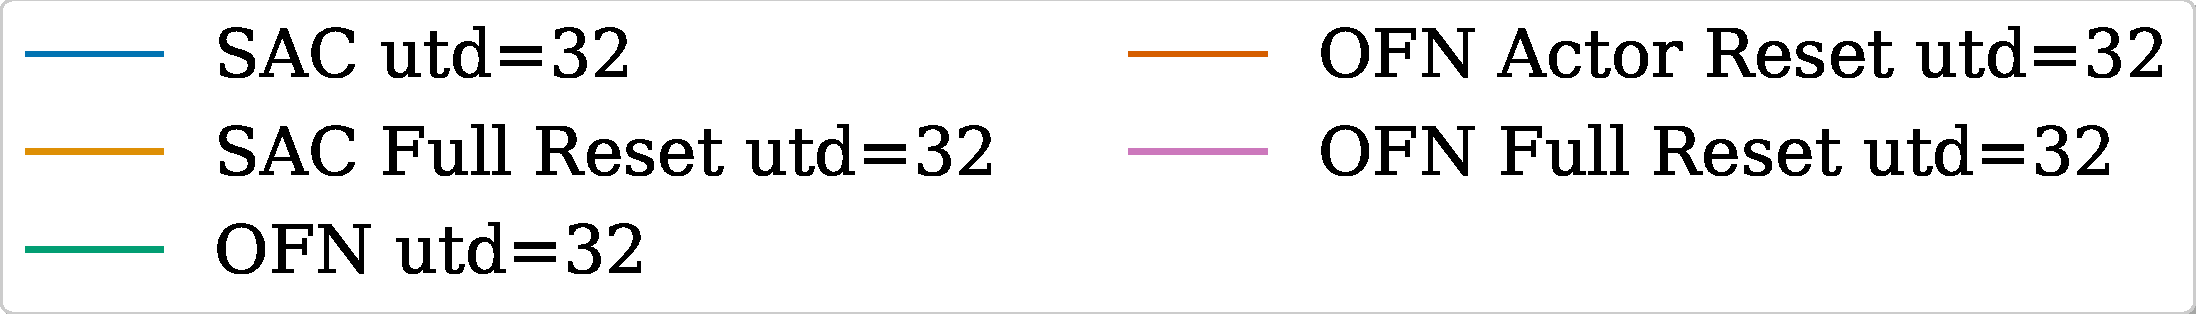
\includegraphics[height=1.1cm]{figures/dissecting/main_exp/utd_32_Q_legend.pdf}
    \end{subfigure}\\%
    \begin{subfigure}[b]{1\textwidth}
        \centering
        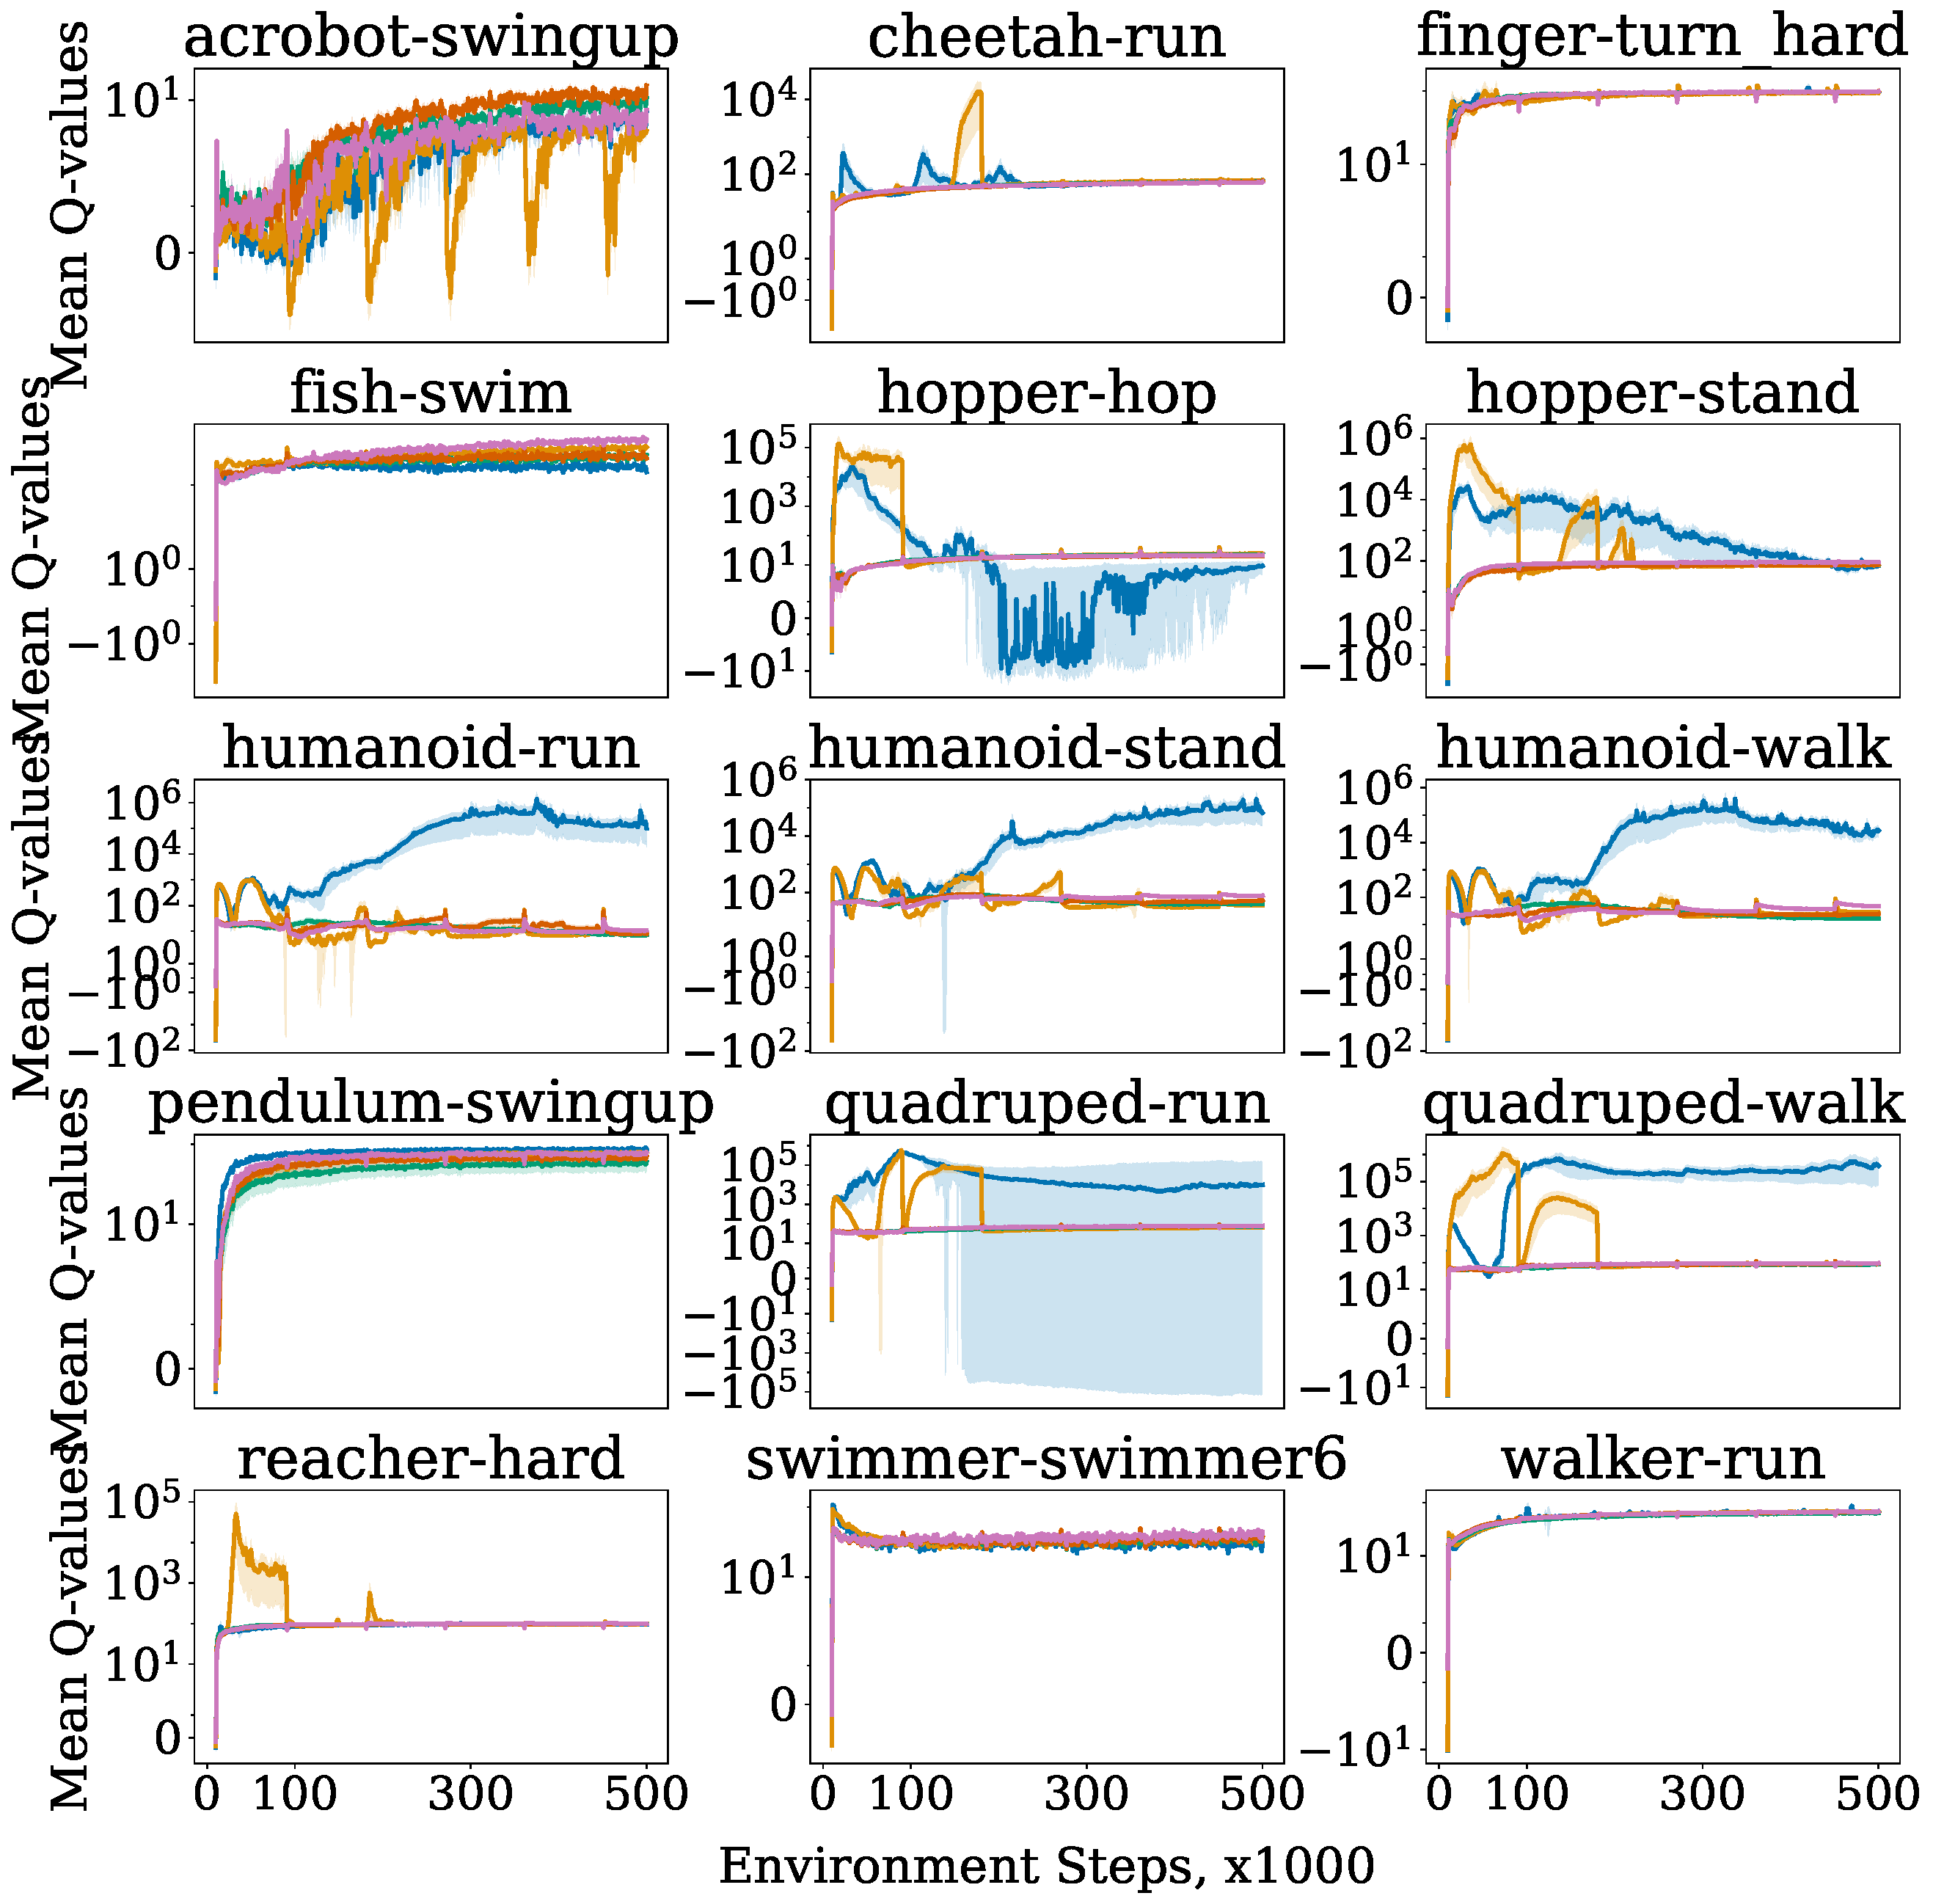
\includegraphics[width=15cm, trim=0cm 0cm 0cm 0cm ,clip]{figures/dissecting/main_exp/utd_32_Q.pdf}
    \end{subfigure}%
    \vspace{-5pt}
    \caption{UTD32 Q-values on Full DMC15-500K. Resetting often works when Q-values diverge. ONF mitigates divergence.}
    % \caption{Mean return, Q-values and Adam moments for priming of different lengths. Dotted lines indicate end of priming. More priming leads to lower return and Q-value and optimizer divergence.}
    \label{fig:utd32_Q}
\end{figure}

\newpage

\section{Unit norm gradient derivation} \label{app:unitnorm}

Here, we take a look at the gradient of the unit norm projection.

Let $i \in {1, ..., N}$, for all $\mathbf{x} = (x_1, ..., x_n) \in \mathbb{R}^n \setminus \{0\}$. Suppose $f(\mathbf{x}) = \cfrac{\mathbf{x}}{\| \mathbf{x} \|}$. 

Then, 
\begin{align*}
    \partial_i f(\mathbf{x}) 
    &= \cfrac{\| \mathbf{x} \| e_i - \mathbf{x} \partial_i \| \cdot \| (\mathbf{x}) }{\|\mathbf{x} \|^2} \\
    &= \cfrac{\| \mathbf{x} \| e_i - \cfrac{x_i}{\|\mathbf{x} \|} \mathbf{x}}{\|\mathbf{x} \|^2} \\
    &= \cfrac{1}{\|\mathbf{x} \|} e_i - \cfrac{x_i}{\|\mathbf{x} \|^3} \mathbf{x}
\end{align*}

Note that the second term can grow quite large if the norm of $\mathbf{x}$ is relatively small. Despite this fact, we are able to remedy the exploding gradients using unit norm projection, likely because gradients are small when the norm is small.

\section{Open Problems and Limitations} \label{app:open}

Feature divergence without regularization is an important problem that contributes substantially to the issues facing high-UTD learning
However, as our experiments show, there are many additional open problems that introducing normalization does not address.

\textbf{Understanding actor issues}~~The resetting experiments in \autoref{fig:aggregate} highlight that a part of the performance impact of high UTD comes from the actor optimization, not the critic optimization, as resetting the actor can boost performance without changing the critic.
Our work does not address this issue, and to the best of our knowledge there are no specific attempts to investigate the actor optimization process in deep actor-critic reinforcement learning.

{\bf RL Optimizer}~~ As the priming experiments show (\autoref{fig:priming_opt}), the update dynamics introduced by momentum terms in modern optimizers can exacerbate existing overestimation problems. 
\textcite{dabney2014adaptive} derives adaptive step-sizes for reinforcement learning from a theoretical perspective, but the resulting optimization rules have not been adapted to Deep Reinforcement Learning to the best of our knowledge.
A recent study by \textcite{asadi2023resetting} shows that resetting the optimizer can have some benefit in the DQN setting, where it can be tied to the hard updates of the target Q network.
In addition, \textcite{lyle2023understanding} show that optimizers like Adam can lead to reduced plasticity of neural networks.
However, our experiments also highlight that without the accelerated optimization of modern optimizers, convergence of the Q value can be prohibitively slow, highlighting the urgent need for stable and fast optimization in RL.

{\bf Conservative Learning for Online RL}~~ Most current actor-critic methods use some form of pessimistic value estimate to combat the overestimation bias inherent in off-policy Q learning. i.e. via the use of a twinned Q network \parencite{fujimoto2018addressing}.
However, this can lead to pessimistic under-exploration \parencite{lan2020maxmin}.
To address this, \textcite{moskovitz2021tactical} propose to tune the relative impact of pessimistic and optimistic exploration for the environments, while \textcite{lee2021sunrise} show that by combining independent critic estimates from ensembles, a UBC like exploration bound can be computed.
These changes could be combined with the mitigation strategies for the feature layer divergence in future work to mitigate the harmful effects of underexploration further.

As our work shows, some of the previous problems with overestimation might not emerge from the bias introduced by off-policy actions, but from the learning dynamics of neural network updates.
This suggests that more work on the exact causes of overestimation might allow us to move beyond the overly pessimistic twinned network minimization trick without needing costly solutions like ensemble methods.

{\bf Tau}~~ The rate of the target network updates is an important hyperparameter in online RL, either through periodic hard copies \parencite{mnih2013playing} or the use of a Polyak averaging scheme \parencite{lillicrap2016ddpg}.
Updating the network too fast can exacerbate the impact of value divergence, while updating too slowly can delay learning. Preliminary experiments show a relationship between value divergence and target update speed that requires further investigation.

There have also been attempts to accelerate optimization not via the neural network optimization, but through adapting the updates of the target networks \parencite{vieillard2020momentum,farahmand2021pid}.
This is an orthogonal direction to the one presented here, and the interplay between target network updates and neural network optimization steps are an important topic for future work.

% We experimented with higher update speeds for the $\tau$ factor in the Polyak averaging scheme of SAC, but were not successful in achieving stable speedup, even after introducing the stabilizing feature normalization.

{\bf Reward Shaping Impact}~~ In several environments, we observe almost no detrimental effects due to high update ratios, while in others the Q-values diverge even without moving beyond one update per sample collected.
A closer inspection suggests that environments in which the initial reward is small and uninformative are much more prone to lead to catastrophic divergence, suggesting a close connection between reward shaping and divergence.
While sparse reward problems have received much attention in the context of exploration, our findings suggests that they also present a challenge for efficient optimization.
Beyond this phenomenon, the interactions between optimization and explorations have been hypothesized to be a strong contributing factor to the good performance of some algorithms \parencite{schaul2022phenomenon}, but the role diverging Q-values play in this phenomenon is to the best of our knowledge mostly unexplored.



